\documentclass[11pt]{article}
\usepackage[T1]{fontenc}
\usepackage{amsmath,amssymb,bm}
\usepackage[margin=1in]{geometry}
\usepackage{booktabs,longtable,array}
\usepackage{graphicx}
\usepackage{float}
\usepackage{tikz}
\usetikzlibrary{arrows.meta}
\usepackage{pgfplots}
\pgfplotsset{compat=1.18}
\usepackage[superscript]{cite}
\usepackage[hidelinks]{hyperref}
\usepackage{tocloft}
\newcommand{\vct}[1]{\bm{#1}}
\newcommand{\sk}{\operatorname{sk}}
\newcommand{\Cov}{\operatorname{Cov}}
\newcommand{\Frame}{\operatorname{Frame}}
\newcommand{\diag}{\operatorname{diag}}
\newcommand{\tr}{\operatorname{tr}}
\newcommand{\rank}{\operatorname{rank}}
\newcommand{\Fun}[1]{\operatorname{#1}}
\newcommand{\norm}[1]{\left\|#1\right\|_2}
\setcounter{tocdepth}{2}
\cftpagenumbersoff{section}
\cftpagenumbersoff{subsection}
\cftpagenumbersoff{subsubsection}
\begin{document}
\begin{titlepage}
\centering
\vspace*{1.5cm}
{\LARGE\bfseries CIS I Assignment 1\\[0.4cm]
Pointer Calibration Design, Implementation, and Validation\par}
\vspace{1.5cm}
{\large Fall 2026\par}
\vfill
\begin{tabular}{p{0.28\textwidth}p{0.55\textwidth}}
Team member name(s): & Zepei Lin, Yue Ge \\[0.8cm]
Student ID(s): & 3323BF, 7A3BD5 \\[0.8cm]
Contact information: & \texttt{zlin97@jh.edu}, \texttt{yge29@jh.edu}
\end{tabular}
\vfill
\noindent\fbox{\parbox{0.86\textwidth}{
\textbf{Academic-integrity statement}\par\medskip
I (we) have followed the rules in completing this assignment.\par\vspace{1.2cm}
Signature(s): \hrulefill
}}
\vfill
\end{titlepage}

\tableofcontents
\clearpage

\section{Introduction}
Optical tracking is used in image-guided navigation to locate an instrument
from markers attached to its rigid body.  The clinically useful point,
however, is the pointer tip, which is not directly observed.  Its position
must be inferred from the marker geometry and the estimated pointer frame.
Manufacturing errors, tracker noise, and small frame rotations can therefore
produce a substantial tip error, especially when the tip is far from the
reference-frame origin.

This assignment requires marker bodies and placements for a pointer, a fixed
calibration object, and a nearby reference.  The marker coordinates are first
refined from repeated tracker observations.  The pointer tip is then calibrated
from simultaneous pointer/calibration poses and a point-sensor reading.
Finally, one simultaneous pointer/nearby observation is used to predict the tip
in the nearby frame at each test pose.  The required performance is
approximately $2\,\mathrm{mm}$ when the pointer is within $45^\circ$ of
vertical.  The solution uses SVD rigid registration, fixed-batch marker
refinement, least-squares tip calibration, and relative-frame prediction;
marker geometry and placement are chosen to improve rotational accuracy while
remaining inside the tracking volume and avoiding collisions\cite{assignment,repo}.

\section{Mathematical Approach}
\subsection{Notation and frame conventions}
Bold lowercase symbols denote three-dimensional column vectors. A star denotes hidden physical ground truth; a hat denotes an estimate. The subscripts $m$, $k$, and $j$ denote marker body, marker, and observation, and the parenthesized superscript $(r)$ denotes refinement iteration. Lengths are in millimeters and angles are in radians. A rigid frame acts on a point as
\begin{equation}
F\vct{x}=R\vct{x}+\vct{p},\qquad
F^{-1}\vct{y}=R^T(\vct{y}-\vct{p}),\qquad R^TR=I,\quad\det R=1.
\end{equation}
Frames are written as $F=\Frame(R,\vct{p})$. The translation is the source-frame origin expressed in the destination frame; it is not generally the tip position. Define $\sk(\vct{u})\vct{v}=\vct{u}\times\vct{v}$.

\begingroup\small
\begin{longtable}{p{0.20\textwidth}p{0.43\textwidth}p{0.28\textwidth}}
\caption{Mathematical symbols and code variables.}\label{tab:symbols}\\
\toprule
Symbol & Meaning & Repository variable \\\midrule
\endfirsthead
\toprule Symbol & Meaning & Repository variable \\\midrule
\endhead
$\vct{a}_{m,k}$ & Nominal marker coordinate in the marker-body frame. & Initial element of \texttt{body.nominal\_marker\_positions}. \\\midrule
$\vct{a}_{m,k}^*$ & Actual marker coordinate in the marker-body frame; $\vct{a}_{m,k}^*=\vct{a}_{m,k}+\Delta\vct{a}_{m,k}$. & \texttt{body.actual\_marker\_positions[k-1].p}. \\\midrule
$\widehat{\vct{a}}_{m,k}^{(r)}$ & Current estimated marker coordinate; $\widehat{\vct{a}}_{m,k}^{(0)}=\vct{a}_{m,k}$. & Current element of \texttt{body.nominal\_marker\_positions}. \\\midrule
$\vct{b}_{m,j,k}$ & Fixed measured coordinate of marker $k$ in tracker-frame observation $j$; it contains the measurement error $\vct{\epsilon}_{b,m,j,k}$. & Stored element \texttt{result.markers[k-1].p}. \\\midrule
$F_{\mathrm{tracker}}$ & Nominal tracker-to-workspace pose. & \texttt{F\_tracker\_approx}; \texttt{trk.F}. \\\midrule
$F_{\mathrm{tracker}}^*$ & Actual tracker-to-workspace pose in one sampling event. & Internal \texttt{F\_actual}. \\\midrule
$F_{mB}$ & Nominal marker-body-to-workspace pose. & \texttt{F\_approx}; \texttt{placed.body.world\_frame}. \\\midrule
$F_{mB}^*$ & Actual marker-body-to-workspace pose. & \texttt{placed.actual\_placement}. \\\midrule
$F_{\mathrm{near}B}$ & Nominal nearby-reference-body-to-workspace pose. & \texttt{F\_near\_approx}; \texttt{near\_placed.body.world\_frame}. \\\midrule
$F_{\mathrm{near}B}^*$ & Actual nearby-reference-body-to-workspace pose. & \texttt{near\_placed.actual\_placement}; validation only. \\\midrule
$\widehat F_{m,j}^{(r)}$ & Estimated marker-body-to-tracker pose. & \texttt{result.frame}. \\\midrule
$\widehat F_{\mathrm{ptr},j}$, $\widehat F_{\mathrm{cal},j}$ & Pointer-to-tracker and calibration-object-to-tracker pose estimates. & \texttt{F\_ptr\_list[j]}, \texttt{F\_cal\_list[j]}. \\\midrule
$\widehat F_{\mathrm{ptr},\mathrm{test}}$ & Pointer-to-tracker estimate from the single Step-8 observation; the subscript $\mathrm{test}$ is introduced here. & \texttt{obs["ptr\_mb"].frame}. \\\midrule
$\widehat F_{\mathrm{near},\mathrm{test}}$ & Nearby-reference-body-to-tracker estimate from the same Step-8 observation. & \texttt{obs["near\_mb"].frame}. \\\midrule
$\widehat F_{\mathrm{ptr/cal},j}$ & Estimated pointer-to-calibration-object pose; $\widehat F_{\mathrm{cal},j}^{-1}\widehat F_{\mathrm{ptr},j}$. & Computed from the two frame lists; no supplied variable. \\\midrule
$\vct{p}_{\mathrm{sensed},j}$ & Actual tip coordinate relative to the calibration sensor, returned for a valid reading. & \texttt{sensed\_tip\_list[j]}. \\\midrule
$\vct{p}_{\mathrm{tip}}$ & Nominal tip coordinate in the pointer frame. & \texttt{ptr\_tip\_approx}; \texttt{pointer.nominal\_tip\_position}. \\\midrule
$\vct{p}_{\mathrm{tip}}^*$ & Actual tip coordinate in the pointer frame. & Internal \texttt{pointer.get\_actual\_tip\_position()}. \\\midrule
$\widehat{\vct{p}}_{\mathrm{tip},j}$ & Tip-coordinate estimate in the pointer frame from observation $j$; $\widehat F_{\mathrm{ptr},j}^{-1}\widehat F_{\mathrm{cal},j}\vct{p}_{\mathrm{sensed},j}$. & Computed from \texttt{F\_ptr\_list[j]}, \texttt{F\_cal\_list[j]}, and \texttt{sensed\_tip\_list[j]}. \\\midrule
$\delta\vct{p}_{\mathrm{tip},j}$, $C_{\widehat p_{\mathrm{tip},j}}$ & Error and covariance of the estimate from observation $j$. & Derived from the two frame-error covariances and sensor error; no supplied variable. \\\midrule
$\delta\vct{p}_{\mathrm{sensed},j}$, $C_{\mathrm{sensed},j}$ & Calibration-sensor perturbation and covariance; negligible in the assignment. & No supplied variable. \\\midrule
$\widehat{\vct{p}}_{\mathrm{tip}}$ & Final calibrated tip-coordinate estimate; the mean of the $N_j$ values $\widehat{\vct{p}}_{\mathrm{tip},j}$. & \texttt{p\_tip\_est}. \\\midrule
$\widehat C_{\mathrm{tip}}$ & Estimated covariance of $\widehat{\vct{p}}_{\mathrm{tip}}$. & \texttt{p\_tip\_cov}. \\\midrule
$\vct{p}_t^*$ & Actual tip coordinate in the workspace at a test pose. & Computed from validation ground truth. \\\midrule
$\widehat{\vct{p}}_t$ & Predicted tip coordinate in the workspace at a test pose. & Student-computed prediction. \\\midrule
$\widehat{\vct{p}}_{t,\mathrm{near}}$ & Predicted tip coordinate in the nearby reference-body frame at a test pose. & Computed from the two Step-8 frame estimates and \texttt{p\_tip\_est}. \\\midrule
$\vct{p}_{t,\mathrm{near}}^*$ & Actual tip coordinate in the nearby reference-body frame at a test pose. & Computed from actual placements and the actual tip for validation only. \\\midrule
$F_t$ & Commanded test pointer pose relative to the workspace. & \texttt{F\_t\_nominal}. \\\midrule
$F_t^*$ & Actual test pointer pose relative to the workspace. & \texttt{test\_placed.actual\_placement}. \\
\bottomrule
\end{longtable}
\endgroup

\begingroup\footnotesize
\setlength{\tabcolsep}{3pt}
\begin{longtable}{>{\raggedright\arraybackslash}p{0.16\textwidth}>{\raggedright\arraybackslash}p{0.17\textwidth}>{\raggedright\arraybackslash}p{0.19\textwidth}>{\raggedright\arraybackslash}p{0.18\textwidth}>{\raggedright\arraybackslash}p{0.20\textwidth}}
\caption{Nominal, estimated, and actual frames.}\label{tab:frames}\\
\toprule
Frame and direction & Nominal & Estimated & Actual & Relation \\\midrule
\endfirsthead
\toprule Frame and direction & Nominal & Estimated & Actual & Relation \\\midrule
\endhead
Tracker to workspace & $F_{\mathrm{tracker}}$ & None specified. & $F_{\mathrm{tracker}}^*$ & $F_{\mathrm{tracker}}^*=F_{\mathrm{tracker}}\Delta F_{\mathrm{tracker}}$. \\\midrule
Marker body to workspace & $F_{mB}$; nearby instance: $F_{\mathrm{near}B}$. & None specified. & $F_{mB}^*$; nearby instance: $F_{\mathrm{near}B}^*$. & $F_{mB}^*=\Delta F_{mB}F_{mB}$ for \texttt{PlaceMarkerBody}. \\\midrule
Calibration object to workspace & $F_{\mathrm{cal}}$; equivalently $F_{mB}$ for the calibration body. & None specified. & $F_{\mathrm{cal}}^*$ & $F_{\mathrm{cal}}^*=F_{\mathrm{cal}}\Delta F_{\mathrm{cal}}$. \\\midrule
Marker body to tracker & $F_{\mathrm{tracker}}^{-1}F_{mB}$. & $\widehat F_{m,j}^{(r)}$; Step-8 instances: $\widehat F_{\mathrm{ptr},\mathrm{test}}$ and $\widehat F_{\mathrm{near},\mathrm{test}}$. & $(F_{\mathrm{tracker}}^*)^{-1}F_{mB}^*$. & $(F_{\mathrm{tracker}}^*)^{-1}F_{mB}^*=(F_{\mathrm{tracker}}\Delta F_{\mathrm{tracker}})^{-1}(\Delta F_{mB}F_{mB})$. During refinement, SVD uses the current $\{\widehat{\vct{a}}_{m,k}^{(r)}\}$ and the fixed observations $\{\vct{b}_{m,j,k}\}$. \\\midrule
Test pointer to workspace & $F_t$ & No direct full-frame estimate; the single simultaneous observation gives $\widehat F_{\mathrm{ptr},\mathrm{test}}$ and $\widehat F_{\mathrm{near},\mathrm{test}}$, which are used to compute $\widehat{\vct{p}}_{t,\mathrm{near}}$. & $F_t^*$ & $F_t^*=F_t\Delta F_t$. \\
\bottomrule
\end{longtable}
\endgroup

\subsection{Marker-body geometry design}
Let $\vct q_{m,k}=\vct a_{m,k}-\overline{\vct a}_m$ denote a marker
coordinate relative to the body centroid.  For a small body rotation
$\vct\alpha_m$ and translation $\vct\epsilon_m$, its tracker-frame displacement
is
\begin{equation}
\delta\vct b_{m,k}
\simeq R
\begin{bmatrix}-\sk(\vct q_{m,k})&I\end{bmatrix}
\begin{bmatrix}\vct\alpha_m\\\vct\epsilon_m\end{bmatrix}.
\end{equation}
Because $R^TR=I$ and $\sum_k\vct q_{m,k}=0$, summing the squared displacements
gives
\begin{equation}
\sum_k\norm{\delta\vct b_{m,k}}^2
\simeq
\vct\alpha_m^TG_m\vct\alpha_m
+N_k\norm{\vct\epsilon_m}^2,
\qquad
G_m=\sum_k\left(\norm{\vct q_{m,k}}^2I
-\vct q_{m,k}\vct q_{m,k}^T\right).
\label{eq:marker-information}
\end{equation}
Marker geometry affects rotational observability through $G_m$; translation
information depends only on the marker count.  The design therefore maximizes
$\lambda_{\min}(G_m)$ and keeps
$\kappa(G_m)=\lambda_{\max}(G_m)/\lambda_{\min}(G_m)$ near one.

All bodies use the vertices of a triangular bipyramid, scaled by
$R_m=\max_k\norm{\vct q_{m,k}}$:
\begin{equation}
\boxed{
\{\vct a_{m,k}\}_{k=1}^{5}
=\left\{
(R_m,0,0),
\left(-\frac{R_m}{2},\pm\frac{\sqrt3R_m}{2},0\right),
(0,0,\pm R_m)
\right\}.}
\label{eq:triangular-bipyramid}
\end{equation}
For this geometry,
\begin{equation}
G_m=R_m^2\diag\!\left(\frac72,\frac72,3\right),
\qquad
\lambda_{\min}(G_m)=3R_m^2,
\qquad
\kappa(G_m)=\frac76.
\label{eq:bipyramid-information}
\end{equation}
This familiar polyhedron is a practical near-optimum, not an unconstrained
numerical optimum.  Any five points satisfying
$\norm{\vct q_{m,k}}\leq R_m$ obey
\begin{equation}
\lambda_{\min}(G_m)
\leq\frac{\tr(G_m)}{3}
=\frac{2}{3}\sum_k\norm{\vct q_{m,k}}^2
\leq\frac{10}{3}R_m^2.
\end{equation}
The selected bipyramid reaches $3R_m^2$, or $90\%$ of this upper bound, while
remaining centered, noncoplanar, and easy to specify.

The three bodies serve different purposes and need not have equal radii.
Published pointer and dynamic-reference designs provide practical examples of
compact tracked-marker layouts \cite{pointerReview,openDRF}.  The primary
notebook design uses
\begin{equation}
\boxed{
R_{\mathrm{ptr}}=30\ \mathrm{mm},\qquad
R_{\mathrm{cal}}=30\ \mathrm{mm},\qquad
R_{\mathrm{near}}=175\ \mathrm{mm}.}
\label{eq:selected-marker-radii}
\end{equation}
The final tip is expressed in the nearby frame.  A small nearby rotation error
$\delta\theta_{\mathrm{near}}$ therefore produces approximately
\begin{equation}
e_{\mathrm{near}}
\approx d_{\mathrm{near-tip}}\,\delta\theta_{\mathrm{near}},
\qquad
\delta\theta_{\mathrm{near}}\propto\frac{1}{R_{\mathrm{near}}}.
\end{equation}
Hence
\begin{equation}
\boxed{e_{\mathrm{near}}\propto
\frac{d_{\mathrm{near-tip}}}{R_{\mathrm{near}}}.}
\label{eq:near-error-ratio}
\end{equation}
The design iteration follows Equation~\ref{eq:near-error-ratio}.  Sensitivity
testing showed that the nearby radius is the dominant factor: a sufficiently
large radius gives very accurate predictions.  However, an oversized nearby
body would obstruct personnel in a practical clinical workspace.  The design
objective is therefore to minimize $R_{\mathrm{near}}$ while retaining the
required core-region accuracy.  Each iteration moves the nearby body as close
to the test region as collision constraints allow, reduces its radius, and
reruns the full pipeline.  A smaller body can be moved closer again, reducing
$d_{\mathrm{near-tip}}$ and partly compensating for the reduced radius.  The
$175\,\mathrm{mm}$ radius is used in the primary run; larger candidates are
compared in Section~\ref{subsec:validation-near-comparison}.

The resulting dimensions and notebook coordinates are
\begin{center}
\begingroup\scriptsize
\setlength{\tabcolsep}{4pt}
\begin{tabular}{lrrrr}
\toprule
Body & $R_m$ [mm] & Marker span $x\times y\times z$ [mm]
& Minimum spacing [mm] & $\lambda_{\min}(G_m)$ [mm$^2$] \\
\midrule
Pointer & 30 & $45.0\times52.0\times60.0$ & 42.4 & 2700 \\
Calibration & 30 & $45.0\times52.0\times60.0$ & 42.4 & 2700 \\
Nearby reference & 175 & $262.5\times303.1\times350.0$ & 247.5 & 91875 \\
\bottomrule
\end{tabular}
\endgroup
\end{center}
\begin{align}
\{\vct a_{\mathrm{ptr},k}\}_{k=1}^{5}
&=\{[30,0,0]^T,[-15,\pm15\sqrt3,0]^T,[0,0,\pm30]^T\}\ \mathrm{mm},\\
\{\vct a_{\mathrm{cal},k}\}_{k=1}^{5}
&=\{[30,0,0]^T,[-15,\pm15\sqrt3,0]^T,[0,0,\pm30]^T\}\ \mathrm{mm},\\
\{\vct a_{\mathrm{near},k}\}_{k=1}^{5}
&=\{[175,0,0]^T,[-87.5,\pm87.5\sqrt3,0]^T,[0,0,\pm175]^T\}\ \mathrm{mm}.
\end{align}
The nominal pointer tip remains
$\vct p_{\mathrm{tip}}=[0,0,-150]^T\,\mathrm{mm}$.

Table~\ref{tab:marker-count-alternatives} gives the requested alternatives in
terms of the body-specific radius $R_m$.

\begingroup\scriptsize
\setlength{\tabcolsep}{3pt}
\begin{longtable}{c p{0.55\textwidth} c c c}
\caption{Marker layouts for four to eight markers.}\label{tab:marker-count-alternatives}\\
\toprule
$N_k$ & Marker coordinates $(x,y,z)$
& Minimum spacing & $\lambda_{\min}(G)$ & $\kappa(G)$ \\\midrule
\endfirsthead
\toprule
$N_k$ & Marker coordinates $(x,y,z)$
& Minimum spacing & $\lambda_{\min}(G)$ & $\kappa(G)$ \\\midrule
\endhead
4 & Regular tetrahedron:
$R_m(1,1,1)/\sqrt3$, $R_m(1,-1,-1)/\sqrt3$,
$R_m(-1,1,-1)/\sqrt3$, $R_m(-1,-1,1)/\sqrt3$
& $\sqrt{8/3}R_m$ & $\frac83R_m^2$ & 1.00 \\\midrule
\textbf{5} & \textbf{Triangular bipyramid: $(R_m,0,0)$,
$(-R_m/2,\pm\sqrt3R_m/2,0)$, $(0,0,\pm R_m)$}
& $\sqrt2R_m$ & $3R_m^2$ & 1.17 \\\midrule
6 & Regular octahedron: $(\pm R_m,0,0)$, $(0,\pm R_m,0)$,
$(0,0,\pm R_m)$
& $\sqrt2R_m$ & $4R_m^2$ & 1.00 \\\midrule
7 & Pentagonal bipyramid: five vertices
$(R_m\cos(2\pi i/5),R_m\sin(2\pi i/5),0)$,
$i=0,\ldots,4$, and two vertices $(0,0,\pm R_m)$
& $2R_m\sin(\pi/5)$ & $\frac92R_m^2$ & 1.11 \\\midrule
8 & Cube: all eight vertices
$(\pm R_m/\sqrt3,\pm R_m/\sqrt3,\pm R_m/\sqrt3)$
& $2R_m/\sqrt3$ & $\frac{16}{3}R_m^2$ & 1.00 \\
\bottomrule
\end{longtable}
\endgroup

The selected five-point row initializes \path{ptr_local_positions},
\path{cal_local_positions}, and \path{near_local_positions}.  The selected
$150\,\mathrm{mm}$ pointer length initializes \path{ptr_tip_approx}.  It is a
design input: the simulator generates the hidden actual tip position around
this nominal coordinate.  The analytic envelope establishes workspace
feasibility; the assigned simulation cases are used only as a validation
check.

Figure~\ref{fig:marker-geometry-design} shows the common polyhedron; each body
scales it by its selected radius $R_m$.

\begin{figure}[H]
\centering
\begin{tikzpicture}[
  >=Latex,
  x={(0.075cm,-0.025cm)},
  y={(-0.060cm,-0.030cm)},
  z={(0cm,0.075cm)}]
\coordinate (O) at (0,0,0);
\coordinate (A) at (80,0,0);
\coordinate (B) at (-40,69.28,0);
\coordinate (C) at (-40,-69.28,0);
\coordinate (D) at (0,0,80);
\coordinate (E) at (0,0,-80);
\draw[gray!65] (A)--(B)--(C)--cycle;
\draw[gray!65] (D)--(A) (D)--(B) (D)--(C);
\draw[gray!65,dashed] (E)--(A) (E)--(B) (E)--(C);
\filldraw[blue!70!black] (A) circle (2.5pt) node[right] {1};
\filldraw[blue!70!black] (B) circle (2.5pt) node[left] {2};
\filldraw[blue!70!black] (C) circle (2.5pt) node[below] {3};
\filldraw[blue!70!black] (D) circle (2.5pt) node[above] {4};
\filldraw[blue!70!black] (E) circle (2.5pt) node[below] {5};
\filldraw[black] (O) circle (1.5pt);
\draw[->,red!75!black,thick] (O)--(100,0,0) node[right] {$x_m$};
\draw[->,green!55!black,thick] (O)--(0,90,0) node[left] {$y_m$};
\draw[->,blue!70!black,thick] (O)--(0,0,90) node[above] {$z_m$};
\node[align=center] at (0,0,105)
  {triangular-bipyramid template for pointer, calibration, and nearby bodies};
\end{tikzpicture}
\caption{Five-marker triangular bipyramid.}
\label{fig:marker-geometry-design}
\end{figure}

\subsection{Workspace placement design}
The simulator imposes three relevant placement constraints: every marker must
remain in the tracking volume, the nearby marker body must remain outside the
pointer test region, and the physical marker spheres must not collide.  The
simulator has no table or optical-occlusion model.  The connecting structure is
therefore treated as transparent.  The assignment does not prescribe a marker
diameter; for collision checks, each marker is modeled as an
$11.8\,\mathrm{mm}$ sphere, matching a commercially available NDI passive
marker \cite{ndiSphere}.

In tracker coordinates, the assignment tracking volume is modeled as
\begin{equation}
1000\leq y_T\leq2200,\qquad
|x_T|,|z_T|\leq h(y_T).
\label{eq:tracking-frustum}
\end{equation}
Here $h(y_T)$ is the available half-width.  It increases linearly from
$500\,\mathrm{mm}$ at the near plane to $1000\,\mathrm{mm}$ at the far plane.
A $50\,\mathrm{mm}$ nominal boundary margin is used.  If a body origin is
$\vct c$ and every marker satisfies $\norm{\vct a_{m,k}}\leq R_m$, then every
orientation lies inside the radius-$R_m$ ball about $\vct c$.  The following
conditions therefore guarantee the margin for all rotations:
\begin{equation}
\boxed{
\begin{aligned}
c_y-R_m&\geq1050,& c_y+R_m&\leq2150,\\
|c_x|+R_m&\leq h(c_y-R_m)-50,&
|c_z|+R_m&\leq h(c_y-R_m)-50.
\end{aligned}}
\label{eq:workspace-envelope}
\end{equation}
This spherical bound is conservative, but it covers continuous orientations
without enumerating the assigned Euler-angle grid.

The tracker is first placed in a side-view configuration, and the calibration
body is fixed to the right of the test region:
\begin{equation}
\boxed{
\begin{aligned}
{}^W\vct p_T&=[300,-1500,300]^T,& {}^WR_T&=I,\\
{}^W\vct p_C&=[730,402,300]^T,& {}^WR_C&=I.
\end{aligned}}
\label{eq:tracker-cal-placement}
\end{equation}
A commanded pointer origin is
\begin{equation}
{}^W\vct p_P=[300+t_x,300+t_y,300+t_z]^T,
\qquad
{}^T\vct p_P=[t_x,1800+t_y,t_z]^T,
\end{equation}
where $t_x,t_y,t_z\in\{0,\pm100,\pm200\}\,\mathrm{mm}$.  With
$R_{\mathrm{ptr}}=30\,\mathrm{mm}$, all pointer markers lie in
$[-230,230]$ in tracker $x$ and $z$, and in $[1570,2030]$ in tracker $y$.
Their minimum frustum clearance is $170\,\mathrm{mm}$.

The nearby placement is selected after choosing its radius.  Its $y$ and $z$
coordinates are aligned with the central nominal tip, and it is moved toward
the test region until the marker centers retain a $30\,\mathrm{mm}$ gap.  For
radius $R_{\mathrm{near}}$, this gives
\begin{equation}
{}^W\vct p_N(R_{\mathrm{near}})
=\left[40-\frac{R_{\mathrm{near}}}{2},\ 300,\ 150\right]^T,
\qquad {}^WR_N=R_z(\pi).
\label{eq:iterated-near-placement}
\end{equation}
This placement rule implements Equation~\ref{eq:near-error-ratio}: reducing the
radius also reduces the body's physical envelope, allowing its origin to move
closer to the test region.  Radius and position are updated together, and the
full pipeline is rerun after each update.  For the primary radius
$R_{\mathrm{near}}=175\,\mathrm{mm}$, the ideal $x_W=-47.5\,\mathrm{mm}$ is
rounded outward to $-48\,\mathrm{mm}$:
\begin{equation}
\boxed{{}^W\vct p_N=[-48,300,150]^T,
\qquad {}^WR_N=R_z(\pi).}
\label{eq:selected-near-placement}
\end{equation}
The final placement is checked directly.  The pointer, calibration, and nearby
markers remain inside the tracking volume, with minimum boundary clearances of
$170.0$, $272.0$, and $248.4\,\mathrm{mm}$, respectively.  The nearby marker
spheres remain outside the test region and retain at least
$18.7\,\mathrm{mm}$ surface clearance from the pointer spheres.  During
calibration, the pointer and calibration spheres retain at least
$73.2\,\mathrm{mm}$ surface clearance.  Therefore the selected placement has
no marker-sphere collisions in the required calibration or test poses.

In Figure~\ref{fig:workspace-coverage}, the red, orange, and green triangular
bipyramids represent the pointer, calibration, and nearby bodies,
respectively.  The blue box bounds the pointer markers over all Step~8 test
poses.

\begin{figure}[H]
\centering
\resizebox{0.96\textwidth}{!}{%
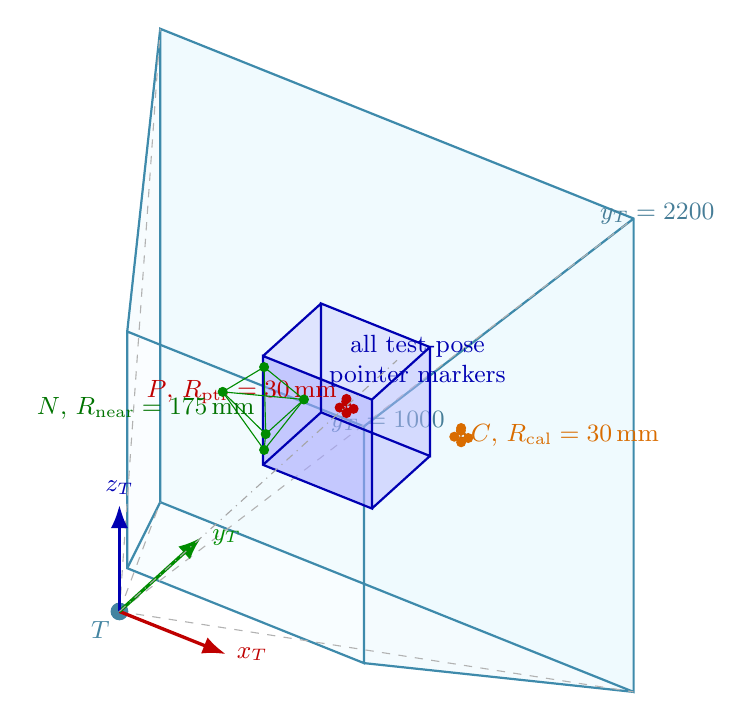
\begin{tikzpicture}[
  >=Latex,
  font=\small,
  x={(0.0030cm,-0.0012cm)},
  y={(0.0016cm,0.00145cm)},
  z={(0cm,0.0030cm)}]
% Tracker and the near/far corners of the square frustum.
\coordinate (T) at (0,0,0);
\coordinate (A) at (-500,1000,-500);
\coordinate (B) at ( 500,1000,-500);
\coordinate (C1) at ( 500,1000, 500);
\coordinate (D) at (-500,1000, 500);
\coordinate (E) at (-1000,2200,-1000);
\coordinate (F) at ( 1000,2200,-1000);
\coordinate (G) at ( 1000,2200, 1000);
\coordinate (H) at (-1000,2200, 1000);

% Transparent frustum faces and edges.
\fill[cyan!18,opacity=0.28] (E)--(F)--(G)--(H)--cycle;
\fill[cyan!12,opacity=0.22] (A)--(B)--(F)--(E)--cycle;
\fill[cyan!12,opacity=0.18] (B)--(C1)--(G)--(F)--cycle;
\fill[cyan!12,opacity=0.16] (D)--(A)--(E)--(H)--cycle;
\fill[cyan!12,opacity=0.12] (C1)--(D)--(H)--(G)--cycle;
\draw[cyan!65!black,thick] (A)--(B)--(C1)--(D)--cycle;
\draw[cyan!65!black,thick] (E)--(F)--(G)--(H)--cycle;
\draw[cyan!65!black,thick] (A)--(E) (B)--(F) (C1)--(G) (D)--(H);
\draw[gray!60,dashed] (T)--(E) (T)--(F) (T)--(G) (T)--(H);
\node[cyan!55!black] at (600,1000,560) {$y_T=1000$};
\node[cyan!55!black] at (1100,2200,1060) {$y_T=2200$};

% Conservative box containing pointer markers over every required test pose.
\coordinate (Q1) at (-230,1570,-230);
\coordinate (Q2) at ( 230,1570,-230);
\coordinate (Q3) at ( 230,1570, 230);
\coordinate (Q4) at (-230,1570, 230);
\coordinate (Q5) at (-230,2030,-230);
\coordinate (Q6) at ( 230,2030,-230);
\coordinate (Q7) at ( 230,2030, 230);
\coordinate (Q8) at (-230,2030, 230);
\fill[blue!35,opacity=0.60] (Q1)--(Q2)--(Q3)--(Q4)--cycle;
\fill[blue!28,opacity=0.48] (Q2)--(Q6)--(Q7)--(Q3)--cycle;
\fill[blue!22,opacity=0.42] (Q4)--(Q3)--(Q7)--(Q8)--cycle;
\draw[blue!70!black,thick]
  (Q1)--(Q2)--(Q3)--(Q4)--cycle
  (Q5)--(Q6)--(Q7)--(Q8)--cycle
  (Q1)--(Q5) (Q2)--(Q6) (Q3)--(Q7) (Q4)--(Q8);
\node[blue!70!black,align=center] at (300,1800,310)
  {all test-pose\\pointer markers};

% Pointer triangular bipyramid at the central test pose.
\draw[red!75!black]
  (30,1800,0)--(-15,1825.98,0)--(-15,1774.02,0)--cycle;
\draw[red!75!black]
  (0,1800,30)--(30,1800,0)
  (0,1800,30)--(-15,1825.98,0)
  (0,1800,30)--(-15,1774.02,0)
  (0,1800,-30)--(30,1800,0)
  (0,1800,-30)--(-15,1825.98,0)
  (0,1800,-30)--(-15,1774.02,0);
\foreach \x/\y/\z in
  {30/1800/0,-15/1825.98/0,-15/1774.02/0,0/1800/30,0/1800/-30}
  \filldraw[red!75!black] (\x,\y,\z) circle (1.6pt);
\node[red!75!black,left] at (0,1800,60)
  {$P$, $R_{\mathrm{ptr}}=30\,\mathrm{mm}$};

% Exact calibration and nearby-reference triangular bipyramids.
\draw[orange!75!black]
  (460,1902,0)--(415,1927.98,0)--(415,1876.02,0)--cycle;
\draw[orange!75!black]
  (430,1902,30)--(460,1902,0)
  (430,1902,30)--(415,1927.98,0)
  (430,1902,30)--(415,1876.02,0)
  (430,1902,-30)--(460,1902,0)
  (430,1902,-30)--(415,1927.98,0)
  (430,1902,-30)--(415,1876.02,0);
\foreach \x/\y/\z in
  {460/1902/0,415/1927.98/0,415/1876.02/0,430/1902/30,430/1902/-30}
  \filldraw[orange!85!black] (\x,\y,\z) circle (1.6pt);
\node[orange!85!black,right] at (430,1902,0)
  {$C$, $R_{\mathrm{cal}}=30\,\mathrm{mm}$};

\draw[green!55!black]
  (-523,1800,-150)--(-260.5,1648.45,-150)--(-260.5,1951.55,-150)--cycle;
\draw[green!55!black]
  (-348,1800,25)--(-523,1800,-150)
  (-348,1800,25)--(-260.5,1648.45,-150)
  (-348,1800,25)--(-260.5,1951.55,-150)
  (-348,1800,-325)--(-523,1800,-150)
  (-348,1800,-325)--(-260.5,1648.45,-150)
  (-348,1800,-325)--(-260.5,1951.55,-150);
\foreach \x/\y/\z in
  {-523/1800/-150,-260.5/1648.45/-150,-260.5/1951.55/-150,-348/1800/25,-348/1800/-325}
  \filldraw[green!55!black] (\x,\y,\z) circle (1.6pt);
\node[green!45!black,left] at (-348,1800,-150)
  {$N$, $R_{\mathrm{near}}=175\,\mathrm{mm}$};

% Tracker-frame axes and centerline.
\filldraw[cyan!60!black] (T) circle (3pt) node[below left] {$T$};
\draw[->,red!75!black,very thick] (T)--(450,0,0) node[right] {$x_T$};
\draw[->,green!55!black,very thick] (T)--(0,650,0) node[right] {$y_T$};
\draw[->,blue!70!black,very thick] (T)--(0,0,450) node[above] {$z_T$};
\draw[gray!70,dash dot] (T)--(0,2200,0);
\end{tikzpicture}%
}
\caption{Marker-body placements in tracker coordinates.}
\label{fig:workspace-coverage}
\end{figure}



In the notebook, ${}^WR_T$ and ${}^W\vct{p}_T$ form
\path{F_tracker_approx}, while ${}^WR_C,{}^W\vct{p}_C$ and
${}^WR_N,{}^W\vct{p}_N$ form the inputs to
\path{simulation.place_marker_body}.  Step~8 constructs the pointer frame from
\path{Rot.xyz(rx,ry,rz)} and $[300+t_x,300+t_y,300+t_z]^T$
\cite{assignment,repo}.

\subsection{Measurement model and origins of uncertainty}
\subsubsection{Error sources and specified limits}
\begingroup\small
\begin{longtable}{p{0.22\textwidth}p{0.38\textwidth}p{0.31\textwidth}}
\caption{Error quantities and limits.}\label{tab:errorlimits}\\
\toprule
Quantity & Bound or model & Value \\\midrule
\endfirsthead
\toprule Quantity & Bound or model & Value \\\midrule
\endhead
Marker positions $\Delta\vct{a}_{m,k}$ & $\norm{\Delta\vct{a}_{m,k}}\leq\delta_{\mathrm{markers}}$ & $\delta_{\mathrm{markers}}$; explicitly $2\,\mathrm{mm}$ for the pointer and calibration object. \\\midrule
Marker body placement $\Delta F_{mB}$ & $F_{mB}^*=\Delta F_{mB}F_{mB}$; $\norm{\vct{\alpha}_{mB}}\leq\delta_{mBa}$, $\norm{\vct{\epsilon}_{mB}}\leq\delta_{mBe}$ & $\delta_{mBa}$ and $\delta_{mBe}$; numerical values not specified. \\\midrule
Calibration object placement $\Delta F_{\mathrm{cal}}$ & $\norm{\vct{\alpha}_{\mathrm{cal}}}\leq0.1$; $\norm{\vct{\epsilon}_{\mathrm{cal}}}\leq25\,\mathrm{mm}$ & $0.1\,\mathrm{rad}$; $25\,\mathrm{mm}$. \\\midrule
Tracker ``jiggle'' $\Delta F_{\mathrm{tracker}}$ & $\norm{\vct{\alpha}_{\mathrm{tracker}}}\leq\sigma_{Ta}$; $\norm{\vct{\epsilon}_{\mathrm{tracker}}}\leq\sigma_{Tp}$ & $\sigma_{Ta}=0.01\,\mathrm{rad}$; $\sigma_{Tp}=5\,\mathrm{mm}$. \\\midrule
Marker measurement error $\vct{\epsilon}_b$ & $C_b=\sigma_b^2I$ & Standard deviation $\sigma_b=0.02\,\mathrm{mm}$; no finite upper bound. \\\midrule
Tracker systematic error & $\Fun{TrackerSystematicError}(\vct{b})=\vct{0}$ & Zero. \\\midrule
Calibration sensor & Returns the actual relative tip position when $\norm{\vct{p}_{\mathrm{sensed}}}\leq5\,\mathrm{mm}$; otherwise returns $[-10000,-10000,-10000]^T$. & Range $5\,\mathrm{mm}$; no sensor-error term. \\\midrule
Test pose $\Delta F_t$ & $F_t^*=F_t\Delta F_t$; $\Delta F_t$ is relatively small & No numerical bound specified. \\\midrule
Tip position error $\Delta\vct{p}_t$ & $\norm{\Delta\vct{p}_t}\leq2\,\mathrm{mm}$ & Required when the pointer is within $45^\circ$ of vertical. \\
\bottomrule
\end{longtable}
\endgroup

\subsubsection{Sensor, hand-guiding, and test placement}
The calibration sensor returns $\vct{p}_{\mathrm{sensed},j}$, the actual pointer-tip position relative to the calibration sensor, when
\begin{equation}
\norm{\vct{p}_{\mathrm{sensed},j}}\leq5\,\mathrm{mm}.
\end{equation}
Otherwise it returns $[-10000,-10000,-10000]^T$. Invalid readings and their paired pose estimates are discarded. No additive sensor-error term is specified.

\subsection{Rigid point-set registration using SVD}
Let $N$ be the number of corresponding marker pairs used in one frame estimate, with $k=1,\ldots,N$. The local marker coordinate $\vct{a}_k$ and measured tracker coordinate $\vct{b}_k$ refer to the same marker. The goal is to find the body-to-tracker rigid transformation
\begin{equation}
F=\Frame(R,\vct{p}),\qquad F\vct{a}_k=R\vct{a}_k+\vct{p},
\end{equation}
that minimizes the total squared point error:
\begin{equation}
\min_{\substack{R^TR=I,\ \det R=1\\\vct{p}}}
\sum_{k=1}^{N}\norm{R\vct{a}_k+\vct{p}-\vct{b}_k}^2.
\end{equation}

First separate translation from rotation. Define the two centroids and subtract them from the points:
\begin{align}
\bar{\vct{a}}&=N^{-1}\sum_k\vct{a}_k,&
\bar{\vct{b}}&=N^{-1}\sum_k\vct{b}_k,\\
\widetilde{\vct{a}}_k&=\vct{a}_k-\bar{\vct{a}},&
\widetilde{\vct{b}}_k&=\vct{b}_k-\bar{\vct{b}}.
\end{align}
For any fixed $R$, the least-squares translation maps the first centroid to the second:
\begin{equation}
\vct{p}=\bar{\vct{b}}-R\bar{\vct{a}}.
\end{equation}
Substitution removes $\vct{p}$ from the remaining problem. Using $R^TR=I$, the rotation-dependent objective becomes
\begin{align}
\sum_{k=1}^{N}\norm{R\widetilde{\vct{a}}_k-\widetilde{\vct{b}}_k}^2
&=\sum_k\norm{\widetilde{\vct{a}}_k}^2
  +\sum_k\norm{\widetilde{\vct{b}}_k}^2
  -2\sum_k\widetilde{\vct{b}}_k^TR\widetilde{\vct{a}}_k.
\end{align}
The first two terms do not depend on $R$. The remaining cross term is collected in the $3\times3$ matrix
\begin{equation}
H=\sum_{k=1}^{N}\widetilde{\vct{a}}_k\widetilde{\vct{b}}_k^T.
\end{equation}
Equivalently, for $r,s\in\{1,2,3\}$,
\begin{equation}
H_{rs}=\sum_{k=1}^{N}
\widetilde a_{k,r}\widetilde b_{k,s}.
\end{equation}
Using $\vct{x}^T\vct{y}=\tr(\vct{y}\vct{x}^T)$ and the cyclic property of the trace,
\begin{equation}
\sum_k\widetilde{\vct{b}}_k^TR\widetilde{\vct{a}}_k
=\tr\!\left(
R\sum_k\widetilde{\vct{a}}_k\widetilde{\vct{b}}_k^T
\right)
=\tr(RH).
\end{equation}
Therefore,
\begin{equation}
\underset{R^TR=I,\ \det R=1}{\operatorname{arg\,min}}
\sum_k\norm{R\widetilde{\vct{a}}_k-\widetilde{\vct{b}}_k}^2
=
\underset{R^TR=I,\ \det R=1}{\operatorname{arg\,max}}
\tr(RH).
\end{equation}

The SVD step begins by decomposing $H$:
\begin{equation}
H=USV^T,\qquad
S=\diag(\sigma_1,\sigma_2,\sigma_3),\qquad
\sigma_1\geq\sigma_2\geq\sigma_3\geq0.
\end{equation}
Writing
\begin{equation}
U=\begin{bmatrix}\vct{u}_1&\vct{u}_2&\vct{u}_3\end{bmatrix},
\qquad
V=\begin{bmatrix}\vct{v}_1&\vct{v}_2&\vct{v}_3\end{bmatrix},
\end{equation}
the singular vectors satisfy
\begin{align}
HH^T\vct{u}_i&=\sigma_i^2\vct{u}_i,&
H^TH\vct{v}_i&=\sigma_i^2\vct{v}_i,
\qquad i=1,2,3,
\end{align}
with $U^TU=I$ and $V^TV=I$.
Substitute the SVD of $H$ into the trace objective and use
$\tr(ABCD)=\tr(DABC)$:
\begin{align}
\tr(RH)
&=\tr(RUSV^T)\\
&=\tr(V^TRUS).
\end{align}
Define
\begin{equation}
W=V^TRU.
\end{equation}
Because $R$, $U$, and $V$ are orthogonal,
\begin{equation}
W^TW=I,\qquad
\det(W)=\det(VU^T)\in\{-1,1\}.
\end{equation}
The determinant condition is not used to expand the trace. Since $S$ is diagonal, $(WS)_{ii}=W_{ii}\sigma_i$. Therefore,
\begin{equation}
\tr(RH)=\tr(WS)
=\sigma_1W_{11}+\sigma_2W_{22}+\sigma_3W_{33}.
\end{equation}
The determinant condition is used only when maximizing this expression. From $W^TW=I$, each column has unit length:
\begin{equation}
\sum_{r=1}^{3}W_{ri}^2=1,\qquad i=1,2,3.
\end{equation}
Therefore every entry satisfies $\lvert W_{ri}\rvert\leq1$. Since $\sigma_i\geq0$,
\begin{equation}
\tr(WS)
=\sum_{i=1}^{3}\sigma_iW_{ii}
\leq\sum_{i=1}^{3}\sigma_i.
\end{equation}
The upper bound is reached by $W=I$. Therefore, if
$\det(VU^T)=1$, $W=I$ is admissible and is a maximizer:
\begin{equation}
\tr(WS)=\sigma_1+\sigma_2+\sigma_3.
\end{equation}
If $\det(VU^T)=-1$, $W=I$ is not admissible because $\det(W)$ must also be $-1$. The determinant-constrained maximum reverses the singular-vector direction associated with the smallest singular value $\sigma_3$.

After computing $U$ and $V$, form the correction matrix
\begin{equation}
D=
\begin{bmatrix}
1&0&0\\
0&1&0\\
0&0&\det(VU^T)
\end{bmatrix}.
\end{equation}
Thus $D=I$ when $\det(VU^T)=1$, and $D_{33}=-1$ when $\det(VU^T)=-1$. The rotation is then computed directly as
\begin{equation}
\boxed{\widehat R=VDU^T.}
\end{equation}
Use this rotation to recover the translation and body-to-tracker frame:
\begin{equation}
\boxed{
\widehat{\vct{p}}=\bar{\vct{b}}-\widehat R\bar{\vct{a}},
\qquad
\widehat F=\Frame(\widehat R,\widehat{\vct{p}}).}
\end{equation}

Point correspondences must be preserved. At least three noncollinear point pairs are required; the assignment notebook requires at least four noncoplanar markers.

In the repository, \texttt{Tracker.procrustes\_solver} implements this SVD calculation. \texttt{simulation.sample\_marker\_bodies} calls it using the current \texttt{nominal\_marker\_positions} and the measured marker coordinates, and returns the resulting body-to-tracker frame as \texttt{result.frame}.

\subsection{Marker geometry refinement}
Let marker body $m$ contain $N_k$ markers.  Collect $N_j$ tracker observations
once and keep their measured coordinates $\vct{b}_{m,j,k}$ fixed throughout
the $N_r$ refinement iterations.  The indices are
\[
k=1,\ldots,N_k,\qquad
j=1,\ldots,N_j,\qquad
r=0,\ldots,N_r-1.
\]
The unknown local marker coordinates and the pose associated with each stored
observation are fitted to the single least-squares objective
\begin{equation}
\mathcal J_m
=
\sum_{j=1}^{N_j}\sum_{k=1}^{N_k}
\norm{
F_{m,j}\vct{a}_{m,k}
-\vct{b}_{m,j,k}
}^2.
\end{equation}
Initialize the estimated local marker coordinates with the nominal model:
\begin{equation}
\widehat{\vct{a}}_{m,k}^{(0)}=\vct{a}_{m,k}.
\end{equation}
Each iteration alternates between the two groups of unknowns.  First, use the
current marker model and the same stored observation $j$ to recompute its
body-to-tracker frame:
\begin{equation}
\widehat F_{m,j}^{(r)}
=
\underset{F}{\operatorname{arg\,min}}
\sum_{k=1}^{N_k}
\norm{
F\widehat{\vct{a}}_{m,k}^{(r)}
-\vct{b}_{m,j,k}
}^2
=
\Frame(\widehat R_{m,j}^{(r)},\widehat{\vct{p}}_{m,j}^{(r)}).
\end{equation}
This is the SVD registration from Section~2.5.  Second, hold the $N_j$
recomputed frames fixed.  The inverse transformation of marker $k$ is
\begin{equation}
(\widehat F_{m,j}^{(r)})^{-1}\vct{b}_{m,j,k}
=
(\widehat R_{m,j}^{(r)})^T
\left(
\vct{b}_{m,j,k}
-\widehat{\vct{p}}_{m,j}^{(r)}
\right).
\end{equation}
All $N_j$ inverse-transformed values correspond to the same local marker
coordinate.  Update marker $k$ by solving
\begin{equation}
\widehat{\vct{a}}_{m,k}^{(r+1)}
=
\underset{\vct{a}}{\operatorname{arg\,min}}
\sum_{j=1}^{N_j}
\norm{
\vct{a}
-
(\widehat F_{m,j}^{(r)})^{-1}
\vct{b}_{m,j,k}
}^2.
\end{equation}
Differentiating with respect to $\vct{a}$ gives
\begin{equation}
2\sum_{j=1}^{N_j}
\left[
\vct{a}
-
(\widehat F_{m,j}^{(r)})^{-1}
\vct{b}_{m,j,k}
\right]
=\vct{0}.
\end{equation}
Therefore,
\begin{equation}
\boxed{
\begin{aligned}
\widehat{\vct{a}}_{m,k}^{(r+1)}
&=
\frac{1}{N_j}
\sum_{j=1}^{N_j}
(\widehat F_{m,j}^{(r)})^{-1}
\vct{b}_{m,j,k}\\
&=
\frac{1}{N_j}
\sum_{j=1}^{N_j}
(\widehat R_{m,j}^{(r)})^T
\left(
\vct{b}_{m,j,k}
-\widehat{\vct{p}}_{m,j}^{(r)}
\right).
\end{aligned}}
\end{equation}
Both steps minimize the same fixed-data objective.  Therefore the objective
cannot increase after either block update:
\begin{equation}
\mathcal J_m(\widehat{\vct{a}}^{(r+1)},\widehat F^{(r)})
\leq
\mathcal J_m(\widehat{\vct{a}}^{(r)},\widehat F^{(r)})
\leq
\mathcal J_m(\widehat{\vct{a}}^{(r)},\widehat F^{(r-1)}).
\end{equation}
After $N_r$ iterations, the output is
$\{\widehat{\vct{a}}_{m,k}^{(N_r)}\}_{k=1}^{N_k}$.  As in any joint
point-set/pose fit, a common rigid change of the body coordinate system is a
gauge freedom; comparisons of marker geometry therefore remove this common
rigid alignment.

In the implementation, $N_j$ is \path{n_readings} and $N_r$ is
\path{passes}.  The $N_j$ calls to
\path{simulation.sample_marker_bodies} occur once before the iteration loop,
so the acquisition count is $N_j$, independent of $N_r$.  At iteration $r$,
\path{Tracker.procrustes_solver} recomputes every
$\widehat F_{m,j}^{(r)}$ from the current marker model and the stored
\path{result.markers}; the stored \path{result.frame} is not reused.  The
fixed measurements are then inverse-transformed, averaged for each marker,
and installed together with \path{placed.body.set_marker_positions}
\cite{assignment,repo}.

\subsection{Sensor-based tip calibration}
For the $N_j$ valid calibration observations, let
$j=1,\ldots,N_j$. In observation $j$, the pointer has desired orientation
$R_{\mathrm{desired},j}$. The quantities used for calibration are the
simultaneously estimated poses $\widehat F_{\mathrm{ptr},j}$ and
$\widehat F_{\mathrm{cal},j}$, together with the sensor coordinate
$\vct{p}_{\mathrm{sensed},j}$. An observation is retained only when
$\norm{\vct{p}_{\mathrm{sensed},j}}\leq 5\,\mathrm{mm}$ \cite{assignment}.

Use both poses from the same observation and define
\begin{equation}
\widehat F_{\mathrm{ptr/cal},j}=\widehat F_{\mathrm{cal},j}^{-1}\widehat F_{\mathrm{ptr},j}
=\Frame(\widehat R_{\mathrm{ptr/cal},j},\widehat{\vct{p}}_{\mathrm{ptr/cal},j}).
\end{equation}
Its components are
\begin{align}
\widehat R_{\mathrm{ptr/cal},j}
&=\widehat R_{\mathrm{cal},j}^T\widehat R_{\mathrm{ptr},j},\\
\widehat{\vct{p}}_{\mathrm{ptr/cal},j}
&=\widehat R_{\mathrm{cal},j}^T
(\widehat{\vct{p}}_{\mathrm{ptr},j}-\widehat{\vct{p}}_{\mathrm{cal},j}).
\end{align}

Expressing the pointer tip in the calibration-object frame gives
\begin{equation}
\widehat R_{\mathrm{ptr/cal},j}\vct{p}_{\mathrm{tip}}+\widehat{\vct{p}}_{\mathrm{ptr/cal},j}
\simeq\vct{p}_{\mathrm{sensed},j}.
\end{equation}
The equal-weight objective is
\begin{equation}
\widehat{\vct{p}}_{\mathrm{tip}}
=\underset{\vct{p}}{\operatorname{arg\,min}}
\sum_j\norm{\widehat R_{\mathrm{ptr/cal},j}\vct{p}
+\widehat{\vct{p}}_{\mathrm{ptr/cal},j}
-\vct{p}_{\mathrm{sensed},j}}^2.
\end{equation}
This is a linear least-squares problem of the form used for pointing-device
calibration in the course notes \cite{calibration,leastsquares}.
Stack the equations as
\begin{equation}
A=\begin{bmatrix}\widehat R_{\mathrm{ptr/cal},1}\\\vdots\\\widehat R_{\mathrm{ptr/cal},N_j}\end{bmatrix},\qquad
\vct{B}=\begin{bmatrix}\vct{p}_{\mathrm{sensed},1}-\widehat{\vct{p}}_{\mathrm{ptr/cal},1}\\\vdots\\
\vct{p}_{\mathrm{sensed},N_j}-\widehat{\vct{p}}_{\mathrm{ptr/cal},N_j}\end{bmatrix}
\end{equation}
\begin{equation}
A\widehat{\vct{p}}_{\mathrm{tip}}\simeq\vct{B},\qquad
\widehat{\vct{p}}_{\mathrm{tip}}
=\underset{\vct{p}}{\operatorname{arg\,min}}
\norm{A\vct{p}-\vct{B}}^2.
\end{equation}
\begin{align}
A^TA
&=\sum_{j=1}^{N_j}
\widehat R_{\mathrm{ptr/cal},j}^T
\widehat R_{\mathrm{ptr/cal},j}
=N_jI,\\
A^T\vct{B}
&=\sum_{j=1}^{N_j}
\widehat R_{\mathrm{ptr/cal},j}^T
(\vct{p}_{\mathrm{sensed},j}-\widehat{\vct{p}}_{\mathrm{ptr/cal},j}).
\end{align}
Therefore,
\begin{equation}
\boxed{
\widehat{\vct{p}}_{\mathrm{tip}}
=(A^TA)^{-1}A^T\vct{B}
=\frac1{N_j}\sum_{j=1}^{N_j}
\widehat R_{\mathrm{ptr/cal},j}^T
(\vct{p}_{\mathrm{sensed},j}-\widehat{\vct{p}}_{\mathrm{ptr/cal},j})
}.
\end{equation}
To verify that this least-squares solution is unique and numerically
well-conditioned, use
\begin{equation}
\rank(A)=3,\qquad
\sigma_1(A)=\sigma_2(A)=\sigma_3(A)=\sqrt{N_j}.
\end{equation}

In the implementation, \path{simulation.hand_guide_pointer} places the pointer
for observation $j$ and returns \path{hg_j}. One call to
\path{simulation.sample_marker_bodies} obtains the paired estimates
$\widehat F_{\mathrm{ptr},j}$ and $\widehat F_{\mathrm{cal},j}$, and
\path{simulation.sense_tip(ptr, hg_j)} obtains
$\vct{p}_{\mathrm{sensed},j}$. An invalid sensor result is discarded together
with its two pose estimates. After $N_j$ valid observations have been collected,
\path{numpy.linalg.lstsq} solves the stacked system above. The template function
\path{compute_pivot_calibration} currently accepts only the two pose lists; this
method also requires the corresponding list of sensor coordinates.

\subsection{Single-observation test prediction}
For each test pose, one simultaneous observation provides
$\{\vct{b}_{\mathrm{ptr},\mathrm{test},k}\}$ and
$\{\vct{b}_{\mathrm{near},\mathrm{test},k}\}$ in the tracker frame.  For
$m\in\{\mathrm{ptr},\mathrm{near}\}$, SVD with the final marker model gives
\begin{equation}
\widehat F_{m,\mathrm{test}}
=\Frame(\widehat R_{m,\mathrm{test}},
\widehat{\vct{p}}_{m,\mathrm{test}}),
\qquad
(\widehat R_{m,\mathrm{test}},\widehat{\vct{p}}_{m,\mathrm{test}})
=\underset{R^TR=I,\,\det R=1,\,\vct{p}}{\operatorname{arg\,min}}
\sum_k
\norm{
R\widehat{\vct{a}}_{m,k}^{(N_r)}+\vct{p}
-\vct{b}_{m,\mathrm{test},k}}^2.
\end{equation}
The predicted tip coordinate in the nearby-reference-body frame is
\begin{equation}
\boxed{
\widehat{\vct{p}}_{t,\mathrm{near}}
=\widehat F_{\mathrm{near},\mathrm{test}}^{-1}
\widehat F_{\mathrm{ptr},\mathrm{test}}
\widehat{\vct{p}}_{\mathrm{tip}}.}
\end{equation}
The validation value and reported error are
\begin{equation}
\vct{p}_{t,\mathrm{near}}^*
=(F_{\mathrm{near}B}^*)^{-1}F_t^*\vct{p}_{\mathrm{tip}}^*,
\qquad
\delta\vct{p}_{t,\mathrm{near}}
=\vct{p}_{t,\mathrm{near}}^*
-\widehat{\vct{p}}_{t,\mathrm{near}}.
\end{equation}

In the notebook, one call to
\path{simulation.sample_marker_bodies(trk, [test_placed, near_placed])}
provides both frame estimates.  The simulator's
\path{test_placed.actual_placement},
\path{near_placed.actual_placement}, and actual tip coordinate are used only
to calculate $\vct{p}_{t,\mathrm{near}}^*$ and
$\delta\vct{p}_{t,\mathrm{near}}$.  Each test pose uses one observation
\cite{assignment,repo}.

\subsection{Error and covariance}
\subsubsection{Frame estimates from refined marker bodies}
\label{subsec:frame-estimate-covariance}
After refinement, the actual marker coordinate and the final estimated marker
coordinate are related by
\begin{equation}
\vct{a}_{m,k}^*
=
\widehat{\vct{a}}_{m,k}^{(N_r)}
+\vct{\epsilon}_{m,k}^{a,(N_r)}.
\end{equation}
Linearizing the measured marker coordinate about the estimated frame and the
final marker model gives
\begin{equation}
\underbrace{
\vct{b}_{m,j,k}
-\widehat F_{m,j}\widehat{\vct{a}}_{m,k}^{(N_r)}
}_{\vct{r}_{m,j,k}\;\text{(residual)}}
\simeq
M_{m,j,k}\vct{\eta}_{m,j}
+\vct{W}_{m,j,k}.
\end{equation}
where
\begin{equation}
\boxed{
M_{m,j,k}
=
\widehat R_{m,j}
\begin{bmatrix}
-\sk(\widehat{\vct{a}}_{m,k}^{(N_r)})&I
\end{bmatrix},
\qquad
\vct{\eta}_{m,j}
=
\begin{bmatrix}
\vct{\alpha}_{m,j}\\
\vct{\epsilon}_{m,j}
\end{bmatrix}.}
\end{equation}
The noise term in this linearized frame-estimation equation is
\begin{equation}
\boxed{
\vct{W}_{m,j,k}
=
\widehat R_{m,j}\vct{\epsilon}_{m,k}^{a,(N_r)}
-\vct{\epsilon}_{b,m,j,k}.}
\end{equation}
It combines the remaining marker-coordinate error after refinement with the
tracker measurement error for marker $k$.
If the marker-model error and tracker measurement error are independent, then
\begin{equation}
C_{W,m,j,k}
=
\widehat R_{m,j}
\Cov\!\left(\vct{\epsilon}_{m,k}^{a,(N_r)}\right)
\widehat R_{m,j}^T+C_b,
\qquad C_b=\sigma_b^2I_3.
\end{equation}
Stacking all $N_k$ marker equations gives
\begin{equation}
\vct{r}_{m,j}
\simeq
M_{m,j}\vct{\eta}_{m,j}+\vct{W}_{m,j},
\qquad
C_{W,m,j}=\Cov(\vct{W}_{m,j}).
\end{equation}
The six entries of $\vct{\eta}_{m,j}$ are the local rotational and
translational correction between the SVD frame estimate and the actual frame.
The SVD registration selects the frame that minimizes
$\norm{\vct{r}_{m,j}}^2$.  At this minimum, another linearized pose correction
cannot reduce the residual, so
\begin{equation}
M_{m,j}^T\vct{r}_{m,j}=0.
\end{equation}
Substitution of the stacked linearized relation gives
\begin{equation}
M_{m,j}^T
\left(M_{m,j}\vct{\eta}_{m,j}+\vct{W}_{m,j}\right)=0,
\qquad
\vct{\eta}_{m,j}
=-M_{m,j}^{\dagger}\vct{W}_{m,j},
\end{equation}
where, for full-column-rank $M_{m,j}$,
\begin{equation}
M_{m,j}^{\dagger}
=
\left(M_{m,j}^TM_{m,j}\right)^{-1}M_{m,j}^T.
\end{equation}
Therefore, the covariance of the pose error after SVD registration is
\begin{equation}
\boxed{
C_{\eta_{m,j}}
\simeq
M_{m,j}^{\dagger}C_{W,m,j}(M_{m,j}^{\dagger})^T.}
\end{equation}
\subsubsection{Tip calibration covariance}
For observation $j$, $\widehat F_{\mathrm{cal},j}$ maps the sensed tip from
the calibration-object frame to the tracker frame, and
$\widehat F_{\mathrm{ptr},j}^{-1}$ then maps it to the pointer frame.  The
resulting single-observation estimate is
\begin{equation}
\boxed{
\widehat{\vct{p}}_{\mathrm{tip},j}
=
\widehat F_{\mathrm{ptr},j}^{-1}
\widehat F_{\mathrm{cal},j}
\vct{p}_{\mathrm{sensed},j}.}
\end{equation}
For propagation of the two SVD frame errors, write
\begin{equation}
F_{\mathrm{ptr},j}^*
=\widehat F_{\mathrm{ptr},j}\Delta F_{\mathrm{ptr},j},
\qquad
F_{\mathrm{cal},j}^*
=\widehat F_{\mathrm{cal},j}\Delta F_{\mathrm{cal},j},
\end{equation}
with
\begin{equation}
\Delta F_{m,j}
\simeq
\Frame\!\left(I+\sk(\vct{\alpha}_{m,j}),\vct{\epsilon}_{m,j}\right),
\qquad
\vct{\eta}_{m,j}
=
\begin{bmatrix}
\vct{\alpha}_{m,j}\\
\vct{\epsilon}_{m,j}
\end{bmatrix},
\quad m\in\{\mathrm{ptr},\mathrm{cal}\}.
\end{equation}
Represent the negligible sensor error by
\begin{equation}
C_{\mathrm{sensed},j}
=\Cov\!\left(\delta\vct{p}_{\mathrm{sensed},j}\right)\simeq0.
\end{equation}
Substitution into
$\vct{p}_{\mathrm{tip}}^*=(F_{\mathrm{ptr},j}^*)^{-1}
F_{\mathrm{cal},j}^*
(\vct{p}_{\mathrm{sensed},j}+\delta\vct{p}_{\mathrm{sensed},j})$
and removal of
second-order terms gives
\begin{equation}
\boxed{
\begin{aligned}
\delta\vct{p}_{\mathrm{tip},j}
:={}&
\vct{p}_{\mathrm{tip}}^*
-\widehat{\vct{p}}_{\mathrm{tip},j}\\
\simeq{}&
\begin{bmatrix}
\sk(\widehat{\vct{p}}_{\mathrm{tip},j})&-I
\end{bmatrix}
\vct{\eta}_{\mathrm{ptr},j}\\
&+
\widehat R_{\mathrm{ptr},j}^T\widehat R_{\mathrm{cal},j}
\begin{bmatrix}
-\sk(\vct{p}_{\mathrm{sensed},j})&I
\end{bmatrix}
\vct{\eta}_{\mathrm{cal},j}\\
&+
\widehat R_{\mathrm{ptr},j}^T\widehat R_{\mathrm{cal},j}
\delta\vct{p}_{\mathrm{sensed},j}.
\end{aligned}}
\end{equation}
If the three error terms are uncorrelated, then
\begin{equation}
\boxed{
\begin{aligned}
C_{\widehat p_{\mathrm{tip},j}}
\simeq{}&
\begin{bmatrix}
\sk(\widehat{\vct{p}}_{\mathrm{tip},j})&-I
\end{bmatrix}
C_{\eta_{\mathrm{ptr},j}}
\begin{bmatrix}
\sk(\widehat{\vct{p}}_{\mathrm{tip},j})&-I
\end{bmatrix}^{T}\\
&+
\widehat R_{\mathrm{ptr},j}^{T}\widehat R_{\mathrm{cal},j}
\begin{bmatrix}
-\sk(\vct{p}_{\mathrm{sensed},j})&I
\end{bmatrix}
C_{\eta_{\mathrm{cal},j}}
\begin{bmatrix}
-\sk(\vct{p}_{\mathrm{sensed},j})&I
\end{bmatrix}^{T}
\widehat R_{\mathrm{cal},j}^{T}\widehat R_{\mathrm{ptr},j}\\
&+
\widehat R_{\mathrm{ptr},j}^{T}\widehat R_{\mathrm{cal},j}
C_{\mathrm{sensed},j}
\widehat R_{\mathrm{cal},j}^{T}\widehat R_{\mathrm{ptr},j}.
\end{aligned}}
\end{equation}
The final calibrated value is
\begin{equation}
\widehat{\vct{p}}_{\mathrm{tip}}
=
\frac{1}{N_j}
\sum_{j=1}^{N_j}
\widehat{\vct{p}}_{\mathrm{tip},j}.
\end{equation}
For independent observations,
\begin{equation}
C_{\widehat p_{\mathrm{tip}}}
\simeq
\frac{1}{N_j^2}
\sum_{j=1}^{N_j}
C_{\widehat p_{\mathrm{tip},j}}.
\end{equation}
This is the covariance obtained by propagating the per-observation
covariances.  The supplied simulator does not compute
$C_{\widehat p_{\mathrm{tip},j}}$, and the template
\path{compute_pivot_calibration} leaves its covariance output for the student
to implement.  The same final covariance can instead be estimated from the
sample variation of the $N_j$ single-observation estimates:
\begin{equation}
\boxed{
\begin{aligned}
\widehat C_{\mathrm{tip}}
={}&
\frac{1}{N_j(N_j-1)}
\sum_{j=1}^{N_j}
\left[
\widehat{\vct{p}}_{\mathrm{tip},j}
-\widehat{\vct{p}}_{\mathrm{tip}}
\right]\\
&\quad{}
\left[
\widehat{\vct{p}}_{\mathrm{tip},j}
-\widehat{\vct{p}}_{\mathrm{tip}}
\right]^T.
\end{aligned}}
\end{equation}

\subsubsection{Single-observation test error}
Using the error notation from
Section~\ref{subsec:frame-estimate-covariance}, the actual relative tip is
\begin{equation}
\vct{p}_{t,\mathrm{near}}^*
=
(\widehat F_{\mathrm{near},\mathrm{test}}
\Delta F_{\mathrm{near},\mathrm{test}})^{-1}
\widehat F_{\mathrm{ptr},\mathrm{test}}
\Delta F_{\mathrm{ptr},\mathrm{test}}
(\widehat{\vct{p}}_{\mathrm{tip}}
+\delta\vct{p}_{\mathrm{tip}}).
\end{equation}
Retaining terms linear in the errors gives
\begin{equation}
\boxed{
\begin{aligned}
\delta\vct{p}_{t,\mathrm{near}}
\simeq{}&
\widehat R_{\mathrm{near},\mathrm{test}}^T
\widehat R_{\mathrm{ptr},\mathrm{test}}
\delta\vct{p}_{\mathrm{tip}}\\
&+\widehat R_{\mathrm{near},\mathrm{test}}^T
\widehat R_{\mathrm{ptr},\mathrm{test}}
\begin{bmatrix}
-\sk(\widehat{\vct{p}}_{\mathrm{tip}})&I
\end{bmatrix}
\vct{\eta}_{\mathrm{ptr},\mathrm{test}}\\
&+\begin{bmatrix}
\sk(\widehat{\vct{p}}_{t,\mathrm{near}})&-I
\end{bmatrix}
\vct{\eta}_{\mathrm{near},\mathrm{test}}.
\end{aligned}}
\end{equation}
Because both frames are estimated from the same observation, the common
tracker pose cancels.

\section{Algorithmic Approach}
The implementation uses Python~3 in a Jupyter notebook.  NumPy is the
principal non-standard numerical library; it is used for array operations,
linear least squares, singular-value and rank checks, covariance calculations,
and numerical validation.  Matplotlib is used to generate the sensitivity
plots.  The Python \path{unittest} module is part of the standard library and
is used for deterministic tests.  The course-provided \path{src} and
\path{data_types} modules supply the simulator and the vector, rotation, frame,
and covariance classes used by the implementation.

The computational pipeline proceeds through marker-body initialization and refinement, calibration-observation collection, least-squares tip calibration, and single-observation tip prediction.

\subsection{Marker-body and workspace initialization (Code Cells 2--4)}
\noindent\textit{Main tasks.} Code Cell 2 defines the three marker-body geometries and nominal pointer tip. Code Cell 3 specifies the tracker, calibration-object, and nearby-reference poses in the workspace. Code Cell 4 constructs and places the bodies, defines the pointer, and creates the tracker.

\begingroup\footnotesize
\begin{longtable}{p{0.09\textwidth}p{0.28\textwidth}p{0.25\textwidth}p{0.27\textwidth}}
\caption{Initialization functions (Cells 2--4).}\label{tab:algorithm-initialization-functions}\\
\toprule
Code cell & Function & Inputs & Outputs \\\midrule
\endfirsthead
\toprule Code cell & Function & Inputs & Outputs \\\midrule
\endhead
2 & \path{triangular_bipyramid_positions(radius_mm)} & Marker-body radius in millimeters. & Five local marker coordinates as \path{vct3} objects. \\\midrule
4 & \path{simulation.define_marker_body(name,positions)} & Body name and nominal local marker coordinates. & A \path{MarkerBody}. \\\midrule
4 & \path{simulation.place_marker_body(body,frame,precision)} & Marker body, nominal workspace frame, and placement precision. & A \path{PlacedBody}. \\\midrule
4 & \path{simulation.define_pointer(name,tip,body)} & Pointer name, nominal tip coordinate, and pointer marker body. & A pointer object. \\\midrule
4 & \path{simulation.create_tracker(name,frame)} & Tracker name and nominal workspace frame. & A tracker object. \\
\bottomrule
\end{longtable}
\endgroup

\begin{enumerate}
\renewcommand{\labelenumi}{\roman{enumi}.}
\item \path{triangular_bipyramid_positions} generates the nominal local marker coordinates from the selected radius.  It implements the five-point construction in Section~2.2:
\[
\begin{aligned}
\{\vct{a}_{m,k}\}_{k=1}^{5}=\{&
[R_m,0,0]^T,\;
[-R_m/2,\sqrt{3}R_m/2,0]^T,\\
&[-R_m/2,-\sqrt{3}R_m/2,0]^T,\;
[0,0,R_m]^T,\;
[0,0,-R_m]^T\}.
\end{aligned}
\]
\item \path{simulation.define_marker_body} converts each coordinate list into a marker-body model.
\item After Code Cell 3 assigns the workspace frames, \path{simulation.place_marker_body} creates the placed calibration, nearby, and pointer bodies.
\item \path{simulation.define_pointer} associates the pointer marker body with its nominal tip coordinate.
\item \path{simulation.create_tracker} creates the tracker used by all subsequent sampling calls.
\end{enumerate}

\subsection{Marker-body refinement (Code Cell 5)}
\noindent\textit{Main task.} Code Cell 5 collects 30 observations once for
each of the pointer, calibration, and nearby bodies.  It then performs three
register--average--update passes over the same fixed batch.  Thus each body
requires 30 tracker samples, independent of the number of refinement passes.

\begingroup\footnotesize
\begin{longtable}{p{0.09\textwidth}p{0.29\textwidth}p{0.25\textwidth}p{0.26\textwidth}}
\caption{Refinement functions (Cell 5).}\label{tab:algorithm-refinement-functions}\\
\toprule
Code cell & Function & Inputs & Outputs \\\midrule
\endfirsthead
\toprule Code cell & Function & Inputs & Outputs \\\midrule
\endhead
5 & \path{_point_matrix(points)} & A sequence of \path{vct3} coordinates. & An $N\times3$ coordinate array. \\\midrule
5 & \path{_validate_marker_geometry(points)} & Local marker coordinates. & No returned value; rejects an invalid geometry. \\\midrule
5 & \path{simulation.sample_marker_bodies(tracker,placed_bodies)} & Tracker and requested placed bodies. & One \path{ObservedBody} per body, containing measured markers and an SVD-estimated body-to-tracker pose. \\\midrule
5 & \path{Tracker.procrustes_solver(points,markers)} & Current local marker model and one stored marker observation. & Recomputed body-to-tracker frame for that observation. \\\midrule
5 & \path{_inverse_average_marker_batch(batch,frames)} & Fixed marker observations and their current fitted frames. & Averaged local marker coordinates. \\\midrule
5 & \path{MarkerBody.set_marker_positions(points)} & Refined local marker coordinates. & No returned value; replaces the nominal marker model. \\\midrule
5 & \path{refine_marker_body(trk,placed,n_readings,passes)} & Tracker and placed body; \path{n_readings=30} is the total fixed-batch size and \path{passes=3} is the number of optimization iterations. & No returned value; refines the body model in place. \\
\bottomrule
\end{longtable}
\endgroup

\begin{enumerate}
\renewcommand{\labelenumi}{\roman{enumi}.}
\item \path{refine_marker_body} collects 30 observations once and controls
three refinement passes over that fixed batch.
\item It first calls \path{_validate_marker_geometry}; this helper uses \path{_point_matrix} to check the local coordinate array.
\item Before the pass loop, \path{simulation.sample_marker_bodies} is called
once for each requested observation, and the measured marker coordinates are
stored.
\item Within each pass, \path{Tracker.procrustes_solver} recomputes the frame
for every stored observation using the current marker model:
\[
\widehat F_{m,j}^{(r)}
=
\underset{F}{\operatorname{arg\,min}}
\sum_k
\norm{F\widehat{\vct{a}}_{m,k}^{(r)}-\vct{b}_{m,j,k}}^2.
\]
\item \path{_inverse_average_marker_batch} uses these recomputed frames to
transform the fixed measurements back to the body frame and applies
\[
\widehat{\vct{a}}_{m,k}^{(r+1)}
=
\frac{1}{N_j}
\sum_{j=1}^{N_j}
(\widehat F_{m,j}^{(r)})^{-1}
\vct{b}_{m,j,k}.
\]
\item \path{MarkerBody.set_marker_positions} installs the averaged coordinates before the next pass begins.
\end{enumerate}

\subsection{Calibration-observation collection (Code Cell 6)}
\noindent\textit{Main task.} Code Cell 6 collects \path{N_OBSERVATIONS=60} valid, index-aligned triples of pointer pose, calibration-object pose, and sensed tip position.  Each accepted pair of frame estimates comes from one simultaneous tracker sample.

\begingroup\footnotesize
\begin{longtable}{p{0.09\textwidth}p{0.29\textwidth}p{0.25\textwidth}p{0.26\textwidth}}
\caption{Observation-collection functions (Cell 6).}\label{tab:algorithm-acquisition-functions}\\
\toprule
Code cell & Function & Inputs & Outputs \\\midrule
\endfirsthead
\toprule Code cell & Function & Inputs & Outputs \\\midrule
\endhead
6 & \path{simulation.hand_guide_pointer(pointer,ptr_placed,cal_placed,R_desired)} & Pointer, placed pointer, calibration body, and desired orientation. & The hand-guided pointer placement. \\\midrule
6 & \path{simulation.sample_marker_bodies(tracker,placed_bodies)} & Tracker, pointer body, and calibration body. & Simultaneous pointer and calibration \path{ObservedBody} values. \\\midrule
6 & \path{simulation.sense_tip(pointer,hand_guided)} & Pointer and its hand-guided placement. & Tip coordinate in the calibration-object frame, or \path{None}. \\
\bottomrule
\end{longtable}
\endgroup

\begin{enumerate}
\renewcommand{\labelenumi}{\roman{enumi}.}
\item \path{simulation.hand_guide_pointer} first places the pointer at the next desired calibration orientation.
\item \path{simulation.sample_marker_bodies} then estimates the pointer and calibration-object poses from one simultaneous tracker sample.
\item \path{simulation.sense_tip} reads the tip coordinate in the calibration-object frame.  The validity condition from Section~2.7 is
\[
\norm{\vct{p}_{\mathrm{sensed},j}}\leq 5\,\mathrm{mm}.
\]
\item The two poses and sensed tip are appended together only when the sensor reading is valid; the loop continues until 60 accepted triples have been stored.
\end{enumerate}

\subsection{Least-squares pointer-tip calibration (Code Cells 7--8)}
\noindent\textit{Main tasks.} Code Cell 7 uses the 60 valid triples collected in Cell 6 in one stacked least-squares solve, producing the fixed tip estimate and its covariance.  Code Cell 8 converts the covariance diagonal to per-axis standard deviations and reports the calibrated result.  This stage has no iterative passes.

\begingroup\footnotesize
\begin{longtable}{p{0.09\textwidth}p{0.29\textwidth}p{0.25\textwidth}p{0.26\textwidth}}
\caption{Tip-calibration functions (Cells 7--8).}\label{tab:algorithm-calibration-functions}\\
\toprule
Code cell & Function & Inputs & Outputs \\\midrule
\endfirsthead
\toprule Code cell & Function & Inputs & Outputs \\\midrule
\endhead
7 & \path{_frame_is_valid(frame,atol)} & A rigid frame and numerical tolerance. & Boolean frame-validity result. \\\midrule
7 & \path{numpy.linalg.lstsq(A,B,rcond=None)} & Stacked rotation blocks and translated sensor vectors. & Tip solution, residual data, rank, and singular values. \\\midrule
7 & \path{compute_pivot_calibration(F_ptr_list,F_cal_list,sensed_tip_list)} & Corresponding pointer frames, calibration frames, and sensed tip coordinates. & Calibrated tip \path{p_tip_est} and $3\times3$ covariance \path{p_tip_cov}. \\\midrule
8 & \path{numpy.sqrt(numpy.clip(diag,0,None))} & Diagonal of \path{p_tip_cov}. & Per-axis tip standard deviations. \\
\bottomrule
\end{longtable}
\endgroup

\begin{enumerate}
\renewcommand{\labelenumi}{\roman{enumi}.}
\item \path{compute_pivot_calibration} controls the calibration calculation and processes the three aligned input lists.
\item It calls \path{_frame_is_valid} for every retained pointer/calibration frame pair.
\item For each valid observation, \path{compute_pivot_calibration} first forms the relative frame from Section~2.7,
\[
\widehat F_{\mathrm{ptr/cal},j}
=
\widehat F_{\mathrm{cal},j}^{-1}
\widehat F_{\mathrm{ptr},j}.
\]
With $N_j=60$, the observations contribute three equations each, giving $A\in\mathbb{R}^{180\times3}$ and $\vct{B}\in\mathbb{R}^{180}$.  They are passed once to \path{numpy.linalg.lstsq}, which computes
\[
\widehat{\vct{p}}_{\mathrm{tip}}
=
\underset{\vct{p}}{\operatorname{arg\,min}}
\norm{A\vct{p}-\vct{B}}^2.
\]
\item The least-squares solution produces \path{p_tip_est}.  The scatter of the single-observation estimates
$\widehat{\vct{p}}_{\mathrm{tip},j}
=\widehat F_{\mathrm{ptr},j}^{-1}
\widehat F_{\mathrm{cal},j}
\vct{p}_{\mathrm{sensed},j}$
produces \path{p_tip_cov} using the Section~2.9 covariance formula
\[
\widehat C_{\mathrm{tip}}
=
\frac{1}{N_j(N_j-1)}
\sum_{j=1}^{N_j}
(\widehat{\vct{p}}_{\mathrm{tip},j}-\widehat{\vct{p}}_{\mathrm{tip}})
(\widehat{\vct{p}}_{\mathrm{tip},j}-\widehat{\vct{p}}_{\mathrm{tip}})^T.
\]
\item Code Cell 8 clips the covariance diagonal at zero and applies \path{numpy.sqrt} to obtain the per-axis standard deviations.
\end{enumerate}

\subsection{Single-observation tip prediction (Code Cell 9)}
\noindent\textit{Main task.} Code Cell 9 generates 170 representative test poses and predicts the calibrated tip from exactly one simultaneous pointer/nearby tracker sample at each pose.

\begingroup\footnotesize
\begin{longtable}{p{0.09\textwidth}p{0.29\textwidth}p{0.25\textwidth}p{0.26\textwidth}}
\caption{Tip-prediction functions (Cell 9).}\label{tab:algorithm-prediction-functions}\\
\toprule
Code cell & Function & Inputs & Outputs \\\midrule
\endfirsthead
\toprule Code cell & Function & Inputs & Outputs \\\midrule
\endhead
9 & \path{simulation.place_marker_body(body,frame,precision)} & Pointer marker body, nominal test frame, and precise placement mode. & The pointer body at one test pose. \\\midrule
9 & \path{simulation.sample_marker_bodies(tracker,placed_bodies)} & Tracker, test pointer body, and nearby body. & One simultaneous pointer/nearby observation used for prediction. \\\midrule
9 & \path{Frame.inv()} and \path{Frame.__mul__()} & Pointer and nearby frame estimates and calibrated tip. & Predicted tip coordinate in the nearby-reference frame. \\
\bottomrule
\end{longtable}
\endgroup

\begin{enumerate}
\renewcommand{\labelenumi}{\roman{enumi}.}
\item For each test pose, \path{simulation.place_marker_body} places the pointer at the nominal pose.
\item One call to \path{simulation.sample_marker_bodies} observes the pointer and nearby body simultaneously.
\item \path{Frame.inv} and \path{Frame.__mul__} apply the Section~2.8 single-observation prediction
\[
\widehat{\vct{p}}_{t,\mathrm{near}}
=
\widehat F_{\mathrm{near},\mathrm{test}}^{-1}
\widehat F_{\mathrm{ptr},\mathrm{test}}
\widehat{\vct{p}}_{\mathrm{tip}}.
\]
\end{enumerate}

\subsection{Function-level execution flow}
Figure~\ref{fig:function-flow} shows the implemented call sequence. Every box is a function or method that appears in Code Cells 2--9; arrow labels describe the data passed between calls.

\begin{figure}[H]
\centering
\resizebox{\textwidth}{!}{%
\begin{tikzpicture}[
basefun/.style={draw,rounded corners,align=center,font=\scriptsize,minimum height=0.78cm,text width=3.25cm,line width=0.8pt},
initfun/.style={basefun,draw=blue!65!black,fill=blue!8},
reffun/.style={basefun,draw=green!55!black,fill=green!9},
acqfun/.style={basefun,draw=orange!80!black,fill=orange!12},
calfun/.style={basefun,draw=violet!70!black,fill=violet!10},
testfun/.style={basefun,draw=cyan!60!black,fill=cyan!10},
initflow/.style={-{Latex[length=2mm]},thick,blue!65!black},
refflow/.style={-{Latex[length=2mm]},thick,green!55!black},
acqflow/.style={-{Latex[length=2mm]},thick,orange!80!black},
calflow/.style={-{Latex[length=2mm]},thick,violet!70!black},
testflow/.style={-{Latex[length=2mm]},thick,cyan!65!black},
sharedflow/.style={-{Latex[length=2mm]},thick,dashed,blue!55!black},
flowlabel/.style={font=\scriptsize,fill=white,inner sep=1.5pt}
]
\node[anchor=east,font=\scriptsize\bfseries] at (-6.75,-0.8) {Cells 2--4};
\node[initfun] (geom) at (-4.8,0) {\path{triangular_}\\\path{bipyramid_positions}};
\node[initfun] (define) at (0,0) {\path{simulation.define_}\\\path{marker_body}};
\node[initfun] (place) at (4.8,0) {\path{simulation.place_}\\\path{marker_body}};
\node[initfun] (pointer) at (-2.4,-1.6) {\path{simulation.}\\\path{define_pointer}};
\node[initfun] (tracker) at (2.4,-1.6) {\path{simulation.}\\\path{create_tracker}};

\node[anchor=east,font=\scriptsize\bfseries] at (-6.75,-4.25) {Cell 5};
\node[reffun] (refine) at (-4.8,-3.5) {\path{refine_marker_body}};
\node[reffun] (validate) at (0,-3.5) {\path{_validate_}\\\path{marker_geometry}};
\node[reffun] (sampleR) at (4.8,-3.5) {\path{simulation.sample_}\\\path{marker_bodies}};
\node[reffun] (registerR) at (-4.8,-5.0) {\path{Tracker.}\\\path{procrustes_solver}};
\node[reffun] (average) at (0,-5.0) {\path{_inverse_average_}\\\path{marker_batch}};
\node[reffun] (setmarkers) at (4.8,-5.0) {\path{MarkerBody.set_}\\\path{marker_positions}};

\node[anchor=east,font=\scriptsize\bfseries] at (-6.75,-7.0) {Cell 6};
\node[acqfun] (guide) at (-4.8,-7.0) {\path{simulation.hand_}\\\path{guide_pointer}};
\node[acqfun] (sampleC) at (0,-7.0) {\path{simulation.sample_}\\\path{marker_bodies}};
\node[acqfun] (sense) at (4.8,-7.0) {\path{simulation.sense_tip}};

\node[anchor=east,font=\scriptsize\bfseries] at (-6.75,-9.1) {Cells 7--8};
\node[calfun] (calibrate) at (-4.8,-9.1) {\path{compute_pivot_}\\\path{calibration}};
\node[calfun] (framevalid) at (0,-9.1) {\path{_frame_is_valid}};
\node[calfun] (lstsq) at (4.8,-9.1) {\path{numpy.linalg.lstsq}};

\node[anchor=east,font=\scriptsize\bfseries] at (-6.75,-11.2) {Cell 9};
\node[testfun] (placeT) at (-2.4,-11.2) {\path{simulation.place_}\\\path{marker_body}};
\node[testfun] (sampleT) at (2.4,-11.2) {\path{simulation.sample_}\\\path{marker_bodies}};
\node[testfun] (transform) at (2.4,-12.7) {\path{Frame.inv} /\\\path{Frame.__mul__}};

\draw[initflow] (geom) -- (define);
\draw[initflow] (define) -- (place);
\draw[initflow] (define.south) -- (0,-0.85) -- (-2.4,-0.85) -- (pointer.north);
\draw[initflow] (place.south) -- (4.8,-2.55) -- (-4.8,-2.55) -- (refine.north);
\draw[initflow] (tracker.south) -- (2.4,-2.85) -- (-4.8,-2.85) -- (refine.north);

\draw[refflow] (refine) -- (validate);
\draw[refflow] (validate) -- (sampleR);
\draw[refflow] (sampleR.south) -- (4.8,-4.25) --
  node[flowlabel,above] {fixed batch} (-4.8,-4.25) -- (registerR.north);
\draw[refflow] (registerR) -- (average);
\draw[refflow] (average) -- (setmarkers);
\draw[refflow] (setmarkers.east) -- (6.55,-5.0) -- (6.55,-6.05) --
  node[flowlabel,below] {next pass; reuse batch} (-4.8,-6.05) --
  (registerR.south);

\draw[sharedflow] (pointer.west) -- (-6.35,-1.6) -- (-6.35,-7.0) -- (guide.west);
\draw[sharedflow] (tracker.east) -- (7.05,-1.6) -- (7.05,-6.3) -- (0,-6.3) -- (sampleC.north);
\draw[sharedflow] (7.05,-6.3) -- (7.05,-11.2) -- (sampleT.east);

\draw[acqflow] (guide) -- (sampleC);
\draw[acqflow] (sampleC) -- node[flowlabel,above] {paired poses} (sense);
\draw[acqflow] (sense.east) -- (6.55,-7.0) -- (6.55,-8.25) -- node[flowlabel,below] {valid triples} (-4.8,-8.25) -- (calibrate.north);

\draw[calflow] (calibrate) -- (framevalid);
\draw[calflow] (framevalid) -- (lstsq);

\draw[testflow] (placeT) -- (sampleT);
\draw[testflow] (sampleT) -- node[flowlabel,right] {one sample} (transform);
\draw[calflow] (calibrate.west) -- (-6.35,-9.1) -- (-6.35,-13.75) -- node[flowlabel,below] {calibrated tip} (2.4,-13.75) -- (transform.south);
\end{tikzpicture}%
}
\caption{Execution flow (Cells 2--9).}
\label{fig:function-flow}
\end{figure}


\section{Program Structure}
The program is implemented in one notebook and uses the supplied \path{src}
modules for simulation and rigid-body operations.  The organization of the
runtime, test, and sensitivity branches is summarized below.

\subsection{File and module organization}
\begingroup\small
\begin{longtable}{p{0.32\textwidth}p{0.59\textwidth}}
\caption{Program files and modules.}\label{tab:file-organization}\\
\toprule
Location & Responsibility \\\midrule
\endfirsthead
\toprule Location & Responsibility \\\midrule
\endhead
\path{notebooks/assignment1_template.ipynb} & Defines the marker layouts, workspace poses, refinement and calibration functions, Step~8 prediction loop, validation statistics, unit tests, and sensitivity studies. \\\midrule
\path{src/__init__.py} & Exposes the assignment API used by the notebook, including \path{simulation}, \path{vct3}, \path{Rot}, and \path{Frame}. \\\midrule
\path{src/simulation/} & Provides assignment-facing operations for defining and placing bodies, creating the tracker, hand-guiding the pointer, sensing the tip, and sampling marker bodies. \\\midrule
\path{src/marker.py} and \path{src/pointer.py} & Provide the \path{MarkerBody} and \path{Pointer} models and maintain nominal and hidden actual geometry. \\\midrule
\path{src/tracker.py} & Provides noisy marker acquisition and \path{Tracker.procrustes_solver}, the SVD rigid-registration routine used by sampling and validation helpers. \\\midrule
\path{src/utils.py} & Provides covariance-controlled random sampling used by the simulator. \\\midrule
\path{data_types/} & Provides nominal and uncertain vectors, rotations, frames, and covariance types. \\
\bottomrule
\end{longtable}
\endgroup

\subsection{Program hierarchy and outputs}
Figure~\ref{fig:program-output-hierarchy} organizes the notebook by purpose and identifies the result produced by each branch.  Detailed function interfaces and call relationships are given in Tables~\ref{tab:student-runtime-functions}--\ref{tab:test-sensitivity-drivers}.

\begin{figure}[H]
\centering
\resizebox{0.98\textwidth}{!}{%
\begin{tikzpicture}[
root/.style={draw,rounded corners,fill=gray!12,align=center,font=\small\bfseries,text width=5.2cm,minimum height=0.9cm},
group/.style={draw,rounded corners,align=center,font=\small\bfseries,text width=6.4cm,minimum height=0.9cm},
stage/.style={draw,rounded corners,align=left,font=\scriptsize,text width=6.7cm,minimum height=1.05cm,inner sep=5pt},
edge/.style={-{Latex[length=2mm]},thick,gray!70!black},
trunk/.style={thick,gray!70!black}
]
\node[root] (root) at (0,0) {\path{assignment1_template.ipynb}};
\node[group,fill=blue!8,draw=blue!65!black] (pipeline) at (-4.2,-1.6) {Calibration and prediction pipeline\\Code Cells 2--11};
\node[group,fill=orange!9,draw=orange!75!black] (validation) at (4.2,-1.6) {Unit tests and sensitivity studies\\Code Cells 12--24};

\node[stage,fill=blue!6,draw=blue!55!black] (design) at (-4.2,-3.25) {\textbf{Marker design and setup (Cells 2--4)}\\
\textbf{Output:} three five-marker local layouts, the placed bodies, and the tracker.};
\node[stage,fill=green!9,draw=green!55!black] (refinement) at (-4.2,-4.95) {\textbf{Marker refinement (Cell 5)}\\
\textbf{Sampling:} one fixed batch of 30 observations per body; 3 refinement passes reuse that batch.\\
\textbf{Output:} refined nominal marker coordinates and per-marker update magnitudes.};
\node[stage,fill=orange!8,draw=orange!70!black] (observations) at (-4.2,-6.85) {\textbf{Calibration observation collection (Cell 6)}\\
\textbf{Collection:} 60 valid triples.\\
\textbf{Output:} index-aligned \path{F_ptr_list}, \path{F_cal_list}, and \path{sensed_tip_list}.};
\node[stage,fill=violet!10,draw=violet!70!black] (calibration) at (-4.2,-8.75) {\textbf{Tip calibration (Cells 7--8)}\\
\textbf{Input:} all 60 valid triples in one least-squares solve; no iterative passes.\\
\textbf{Output:} \path{p_tip_est}, \path{p_tip_cov}, and the per-axis standard deviations.};
\node[stage,fill=cyan!10,draw=cyan!60!black] (prediction) at (-4.2,-10.65) {\textbf{Step 8 predictions and design comparison (Cells 9--11)}\\
\textbf{Output:} predictions for all 170 poses, including the core poses
($\theta_{\mathrm{tilt}}\leq45^\circ$) and the extended poses
($\theta_{\mathrm{tilt}}>45^\circ$), the ten largest errors, and a comparison
of three nearby-body diameters.};

\node[stage,fill=orange!7,draw=orange!70!black] (tests) at (4.2,-3.45) {\textbf{Deterministic unit tests (Cells 13--14, 18--19, 21--22, and 24)}\\
\textbf{Output:} pass/fail results for 22 tests in seven test classes.};
\node[stage,fill=yellow!12,draw=orange!70!black] (studies) at (4.2,-5.15) {\textbf{Sensitivity studies (Cells 15--17, 20, and 23)}\\
\textbf{Output:} refinement, calibration-count, and frame-error-propagation curves computed over repeated trials.};

\draw[edge] (root.south) -- (0,-0.8) -| (pipeline.north);
\draw[edge] (root.south) -- (0,-0.8) -| (validation.north);

\draw[trunk] (pipeline.south) -- (-8.0,-2.35) -- (-8.0,-10.65);
\draw[edge] (-8.0,-3.25) -- (design.west);
\draw[edge] (-8.0,-4.95) -- (refinement.west);
\draw[edge] (-8.0,-6.85) -- (observations.west);
\draw[edge] (-8.0,-8.75) -- (calibration.west);
\draw[edge] (-8.0,-10.65) -- (prediction.west);

\draw[trunk] (validation.south) -- (8.0,-2.35) -- (8.0,-5.15);
\draw[edge] (8.0,-3.45) -- (tests.east);
\draw[edge] (8.0,-5.15) -- (studies.east);
\end{tikzpicture}%
}
\caption{Program hierarchy and outputs.}
\label{fig:program-output-hierarchy}
\end{figure}

\subsection{Student runtime functions}
Table~\ref{tab:student-runtime-functions} lists every function defined by the notebook before validation begins.  A function with no returned value updates an object in place or raises a documented exception when its input contract is violated.

\begingroup\scriptsize
\begin{longtable}{p{0.055\textwidth}p{0.225\textwidth}p{0.255\textwidth}p{0.335\textwidth}}
\caption{Runtime functions.}\label{tab:student-runtime-functions}\\
\toprule
Cell & Function & Inputs & Output and purpose \\\midrule
\endfirsthead
\toprule Cell & Function & Inputs & Output and purpose \\\midrule
\endhead
2 & \path{triangular_bipyramid_positions(radius_mm)} & Marker-body radius. & Returns five centered, noncoplanar \path{vct3} coordinates used for the pointer, calibration, and nearby bodies. \\\midrule
5 & \path{_point_matrix(points)} & Sequence of \path{vct3} coordinates. & Returns an $N\times3$ floating-point array.  It is reused by geometry validation, refinement reporting, and unit tests. \\\midrule
5 & \path{_validate_marker_geometry(points)} & Local marker-coordinate sequence. & Returns no value; rejects fewer than four points, nonfinite coordinates, or coplanar geometry.  It calls \path{_point_matrix}. \\\midrule
5 & \path{_inverse_average_marker_batch(batch,frames)} & Fixed \path{ObservedBody} values and their frames recomputed from the current marker model. & Returns one averaged local \path{vct3} per marker after inverse-transforming every fixed observation; rejects empty or inconsistent batches. \\\midrule
5 & \path{refine_marker_body(trk,placed,n_readings,passes)} & Tracker, placed body, fixed-batch observation count, and pass count. & Returns no value; samples once, recomputes every observation frame in each pass, averages the fixed batch, and updates the \path{MarkerBody} in place. \\\midrule
7 & \path{_frame_is_valid(frame,atol)} & Candidate \path{Frame} and tolerance. & Returns a Boolean indicating a finite translation and a finite proper rotation. \\\midrule
7 & \path{compute_pivot_calibration(F_ptr_list,F_cal_list,sensed_tip_list)} & Three index-aligned lists of pointer frames, calibration frames, and sensor readings. & Returns \path{p_tip_est} and the $3\times3$ covariance \path{p_tip_cov}; it filters unusable readings, calls \path{_frame_is_valid}, constructs the stacked system, and calls \path{numpy.linalg.lstsq}. \\
\bottomrule
\end{longtable}
\endgroup

\subsection{Validation and sensitivity helper functions}
The nearby-design evaluator is defined in Code Cell~11, and the shared unit-test
and sensitivity helpers are defined in Code Cell~12.  They use isolated test
objects or restore the NumPy random state after execution, so they do not alter
the calibrated model or the primary Step~8 result.

\begingroup\scriptsize
\begin{longtable}{p{0.215\textwidth}p{0.215\textwidth}p{0.205\textwidth}p{0.225\textwidth}}
\caption{Validation and sensitivity helpers.}\label{tab:validation-helper-functions}\\
\toprule
Function & Inputs & Output & Principal caller or purpose \\\midrule
\endfirsthead
\toprule Function & Inputs & Output & Principal caller or purpose \\\midrule
\endhead
\path{_evaluate_near_design} & Diameter, workspace $x$ coordinate, and setup seed. & All-pose and core-region Step~8 statistics. & Rebuilds, refines, and evaluates one nearby-body candidate while replaying the same Step~8 random sequence. \\\midrule
\path{_run_unit_test}, \path{_print_pass_summary} & A \path{TestCase}, failure message, title, and check labels. & Test result and explicit PASS table. & Execute each deterministic test class and stop on failure. \\\midrule
\path{_point_rows}, \path{_unit_marker_observation} & Local points and a known frame. & Coordinate array or exact synthetic marker observation. & Small adapters for refinement tests. \\\midrule
\path{_exact_refinement_result} & Reading count and pass count. & True/refined points and acquisition/registration call counts. & Verifies exact recovery and fixed-batch reuse. \\\midrule
\path{_synthetic_calibration_case} & No input. & Known tip, paired frames, and in-range sensed tips. & Supplies exact calibration fixtures. \\\midrule
\path{_marker_layout_for_count} & Marker count and radius. & Centered 4--8 marker layout. & Builds the tetrahedron, triangular bipyramid, octahedron, pentagonal bipyramid, or cube used in Cell~16. \\\midrule
\path{_aligned_marker_rmse} & Estimated points, actual points, and tracker. & Gauge-aligned marker-position RMSE. & Removes a common rigid gauge before scoring the refined model. \\\midrule
\path{_test_marker_cases}, \path{_test_frame_rmse} & Actual points, seed, model, tracker, and test cases. & Independent noisy observations and test-frame rotation/translation RMSE. & Evaluate a refined model on observations not used for training. \\\midrule
\path{_refinement_trial} & Layout, reading count, pass count, and seed. & Aligned marker, test-rotation, and test-translation errors. & Runs one isolated fixed-batch refinement trial. \\\midrule
\path{_refinement_objective}, \path{_refinement_trace} & Marker model, fixed batch, frames, controls, and seed. & Training residual and per-iteration validation histories. & Check descent and convergence on one continuous optimization trajectory. \\\midrule
\path{_summarize_trials} & Parameter values, trial callback, and seeds. & Trial array, mean, and sample standard deviation. & Shared repeated-trial aggregator. \\\midrule
\path{_calibration_truth}, \path{_perturb_frame} & Observation count, random generator, and noise scales. & Exact calibration data and perturbed frames. & Controlled fixtures for calibration sensitivity. \\\midrule
\path{_frame_noise_tip_trial} & Observation count and seed. & Calibrated-tip error. & Tests averaging of fixed-strength independent frame errors. \\\midrule
\path{_rotation_error_angle}, \path{_frame_error_to_tip_trial} & Estimated/true frames, error scale, seed, and error kind. & Frame-error RMSE and calibrated-tip error. & Propagates rotation or translation error into tip calibration. \\
\bottomrule
\end{longtable}
\endgroup

\subsection{Test classes and sensitivity drivers}
\begingroup\scriptsize
\begin{longtable}{p{0.09\textwidth}p{0.31\textwidth}p{0.50\textwidth}}
\caption{Unit-test classes and sensitivity drivers.}\label{tab:test-sensitivity-drivers}\\
\toprule
Cells & Class or driver & Tested behavior and output \\\midrule
\endfirsthead
\toprule Cells & Class or driver & Tested behavior and output \\\midrule
\endhead
13 & \path{TestExactMarkerRecovery} & Checks exact recovery of five marker coordinates and verifies that 4 observations with 3 passes cause 4 acquisitions and 12 SVD registrations. \\\midrule
14 & \path{TestRefinementInputValidation} & Checks empty and undersized batches, inconsistent observations, coplanar or nonfinite geometry, and invalid refinement controls. \\\midrule
15 & Refinement observation/convergence drivers & Sweeps 1--40 fixed-batch observations and traces iterations 0--8 while checking that the training objective does not increase. \\\midrule
16 & Marker-count sensitivity driver & Compares the 4-, 5-, 6-, 7-, and 8-marker polyhedra at a common $30\,\mathrm{mm}$ radius. \\\midrule
17 & Marker-radius sensitivity driver & Compares radii from 30 to $250\,\mathrm{mm}$ for the five-marker triangular bipyramid. \\\midrule
18 & \path{TestExactTipRecovery} & Checks exact recovery of a known pointer tip. \\\midrule
19 & \path{TestCalibrationInputValidation} & Checks list alignment, frame type and rigidity, finite data, and sensor type. \\\midrule
20 & Calibration-count sensitivity driver & Sweeps 2--60 valid observations with fixed-strength independent frame errors and a $1/\sqrt{N}$ reference. \\\midrule
21 & \path{TestInvalidSensorFiltering} & Checks the assignment sentinel, the valid $5\,\mathrm{mm}$ boundary, and missing/nonfinite readings. \\\midrule
22 & \path{TestMinimumCalibrationObservations} & Checks rejection of zero or one valid reading and acceptance of two valid readings. \\\midrule
23 & Frame-error-propagation drivers & Independently sweep upstream frame rotation and translation errors and report their effect on calibrated-tip error. \\\midrule
24 & \path{TestCalibrationCovariance} & Checks zero covariance for identical estimates and the analytic covariance of a three-sample mean. \\
\bottomrule
\end{longtable}
\endgroup

\subsection{Program outputs}
The notebook reports four groups of results:
\begin{itemize}
\setlength{\itemsep}{2pt}
\item \textbf{Refined geometry:} updated local marker coordinates for the pointer, calibration, and nearby bodies.
\item \textbf{Tip calibration:} \path{p_tip_est}, its covariance \path{p_tip_cov}, and the standard deviation along each pointer-frame axis.
\item \textbf{Step~8 performance:} single-observation predictions and error statistics for the poses whose actual pointer-axis tilt satisfies $\theta_{\mathrm{tilt}}\leq45^\circ$.
\item \textbf{Validation:} nearby-radius comparisons, 22 deterministic unit-test results, and the refinement and calibration sensitivity plots.
\end{itemize}


\section{Validation Approach}
Validation first measures the final Step~8 prediction error over the test
poses and compares nearby-body sizes.  It then tests marker refinement and tip
calibration separately using exact cases, invalid inputs, and sensitivity
studies.  Hidden simulator values are used only to score completed estimates.

\subsection{Step~8 accuracy within $45^\circ$ and nearby-body size}
The nominal Euler-angle components are selected from the assignment set
\begin{equation}
\Theta=\{0,\pm\pi/6,\pm\pi/3,\pm\pi/2\},
\qquad \theta_j\in\Theta.
\end{equation}
For each evaluated pose, the code computes the actual angle
$\theta_{\mathrm{tilt}}$ between the pointer axis and workspace vertical.
Only the $N_{45}=102$ poses satisfying
$\theta_{\mathrm{tilt}}\leq45^\circ$ are used for the required performance
result.  This classification uses the transformed pointer axis rather than any
single Euler-angle component.

Step~8 predicts a different nearby-frame tip
$\widehat{\vct p}_{t,\mathrm{near},i}$ for each pose from one simultaneous
pointer/nearby observation.  Its error is
\begin{equation}
\Delta\vct p_i
=\widehat{\vct p}_{t,\mathrm{near},i}
-\vct p_{t,\mathrm{near},i}^*,
\qquad e_i=\norm{\Delta\vct p_i}.
\end{equation}
Over the $N_{45}$ required poses, the reported scalar measures are
\begin{equation}
\mathrm{RMSE}_{45}=\sqrt{\frac1{N_{45}}\sum_i e_i^2},
\qquad
\rho_{2\mathrm{mm},45}=\frac1{N_{45}}\sum_i
\mathbf1(e_i\leq2\,\mathrm{mm}).
\end{equation}
The nearby-frame error mean and sample covariance are
\begin{equation}
\overline{\Delta\vct p}_{45}
=\frac1{N_{45}}\sum_i\Delta\vct p_i,
\qquad
\widehat C_{\Delta p,45}
=\frac1{N_{45}-1}\sum_i
(\Delta\vct p_i-\overline{\Delta\vct p}_{45})
(\Delta\vct p_i-\overline{\Delta\vct p}_{45})^T.
\end{equation}
The code evaluates these with the vector mean and
\path{numpy.cov(...,ddof=1)}.  This covariance describes empirical error
across different test poses, not repeated measurements at one pose.

For the $350\,\mathrm{mm}$-diameter nearby body,
\begin{equation}
\overline{\Delta\vct p}_{45}
=[0.044,-0.546,0.998]^T\ \mathrm{mm},
\qquad
\widehat C_{\Delta p,45}
=\begin{bmatrix}
0.203&-0.036&-0.049\\
-0.036&0.170&-0.109\\
-0.049&-0.109&0.100
\end{bmatrix}\ \mathrm{mm}^2.
\end{equation}

\begin{table}[H]
\centering
\small
\caption{Step~8 accuracy within $45^\circ$ of vertical.}
\label{tab:validation-end-to-end}
\begin{tabular}{lrrrr}
\toprule
$N_{45}$ & Mean [mm] & RMSE [mm] & Maximum [mm] & Within $2\,\mathrm{mm}$ \\
\midrule
102 & 1.260 & 1.329 & 2.155 & 96.1\% \\
\bottomrule
\end{tabular}
\end{table}
The required poses pass the chosen 95\% empirical criterion, although one
observed error reaches $2.155\,\mathrm{mm}$.

The nearby body strongly affects this error because its rotation acts on the
tip expressed in the nearby frame.  As its size increases, the nearby body is
placed slightly farther from the test workspace to preserve collision
clearance.  In Table~\ref{tab:validation-near-comparison}, $x_W$ denotes the
$x$ coordinate of the nearby frame's origin in the world coordinate system.
The comparison therefore includes both the larger marker-body size and the
corresponding placement adjustment.

\begin{table}[H]
\centering
\footnotesize
\caption{Nearby-body comparison within $45^\circ$ of vertical.}
\label{tab:validation-near-comparison}
\begin{tabular}{rrrrrr}
\toprule
Diameter [mm] & Radius [mm] & $x_W$ [mm] & RMSE [mm] & Maximum [mm] & Within $2\,\mathrm{mm}$ \\
\midrule
350 & 175 & $-48$ & 1.329 & 2.155 & 96.1\% \\
400 & 200 & $-60$ & 1.235 & 2.284 & 97.1\% \\
500 & 250 & $-85$ & 1.022 & 1.890 & 100.0\% \\
\bottomrule
\end{tabular}
\end{table}

\subsection{Unit Test A: marker refinement}
Unit Test A evaluates the \path{refine_marker_body} function, which updates
local marker coordinates from a fixed batch of tracker observations.  Tests
A.1--A.5 assess coordinate recovery, invalid-input handling, convergence, and
sensitivity to the observation count, marker count, and marker-body radius.
For the marker-error metric, the refined model is first SVD-aligned to the true
model to remove differences in rigid coordinate-frame placement:
\begin{equation}
e_{\mathrm{marker}}
=\sqrt{\frac{1}{N_k}\sum_{k=1}^{N_k}
\norm{F_{\mathrm{align}}\widehat{\vct a}_k-\vct a_k^*}^2}.
\end{equation}

\subsubsection*{A.1 Exact marker-coordinate recovery}
Four exact observations of a known five-marker body recover all coordinates
with a maximum error of $3.949\times10^{-14}\,\mathrm{mm}$.  The initial model
is already exact in this deterministic case.  Call counts confirm four tracker
acquisitions and 12 SVD registrations over three passes, verifying that the
same observations are reused and frames are recomputed each pass.

\subsubsection*{A.2 Invalid refinement inputs}
All six invalid-input tests pass.  The implementation rejects an empty
observation batch, fewer than four observed markers, inconsistent marker/frame
structure, coplanar geometry, nonfinite geometry, and invalid reading/pass
controls.  Each case must raise \path{ValueError} rather than return a
misleading refined model.

\subsubsection*{A.3 Observation-count and iteration sensitivity}
\noindent\textbf{A.3.1 Observation-count sensitivity.}
Figure~\ref{fig:validation-marker-observation-count} shows that a larger fixed
batch reduces aligned marker-coordinate RMSE from $0.02521$ to
$0.00395\,\mathrm{mm}$ as the observation count rises from 1 to 40.  The
independent test-frame errors change little in these trials; the improvement
in local marker geometry does not produce a comparable decrease in
single-observation frame error.  Error bars in the refinement figures are
sample standard deviations across eight seeds, not confidence intervals.

The five-marker triangular bipyramid has radius $30\,\mathrm{mm}$ and is
refined for three passes.  Each plotted point is the eight-seed mean of the
marker RMSE after alignment to the true geometry.

\begin{figure}[H]
\centering
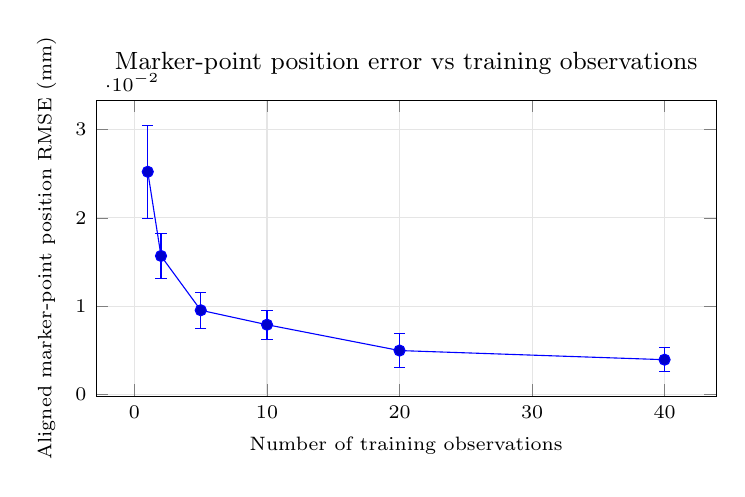
\begin{tikzpicture}
\begin{axis}[
  width=0.78\textwidth,height=0.44\textwidth,
  title={Marker-point position error vs training observations},
  xlabel={Number of training observations},
  ylabel={Aligned marker-point position RMSE (mm)},
  grid=major,grid style={gray!20},
  title style={font=\small},label style={font=\scriptsize},
  tick label style={font=\scriptsize}]
\addplot+[blue,mark=*,error bars/.cd,y dir=both,y explicit]
table[x=x,y=y,y error=err] {
x y err
1  0.025205964 0.005261500
2  0.015682660 0.002575888
5  0.009537215 0.002012480
10 0.007902402 0.001638685
20 0.004979382 0.001911033
40 0.003946139 0.001342286
};
\end{axis}
\end{tikzpicture}
\caption{Marker error versus observation count (A.3.1).}
\label{fig:validation-marker-observation-count}
\end{figure}

\noindent\textbf{A.3.2 Iteration convergence.}
The convergence test reuses one ten-observation batch.  The first pass reduces
the training residual from $1.718717$ to $0.025804\,\mathrm{mm}$ and marker
RMSE from $1.718247$ to $0.007902\,\mathrm{mm}$.  The largest later residual
increase is $1.651\times10^{-14}\,\mathrm{mm}$, consistent with roundoff.
Figure~\ref{fig:validation-refinement-convergence} displays this rapid initial
decrease on a logarithmic scale.  The residual is nearly unchanged after the
second update, supporting three passes for this tested configuration.
Additional passes reuse the same observations and should not be interpreted as
additional independent measurements.

Each trial starts from a perturbed marker model and performs eight updates;
iteration zero denotes the initial model.  The plotted quantity is the mean
training marker-residual RMS across eight seeds, with one sample standard
deviation shown by the error bars.

\begin{figure}[H]
\centering
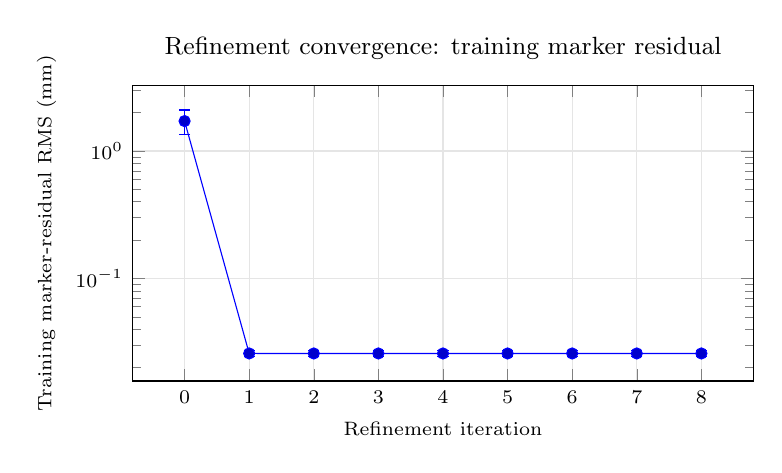
\begin{tikzpicture}
\begin{axis}[
  width=0.78\textwidth,height=0.44\textwidth,
  title={Refinement convergence: training marker residual},
  xlabel={Refinement iteration},
  ylabel={Training marker-residual RMS (mm)},
  ymode=log,xtick={0,1,2,3,4,5,6,7,8},
  grid=major,grid style={gray!20},
  title style={font=\small},label style={font=\scriptsize},
  tick label style={font=\scriptsize}]
\addplot+[blue,mark=*,error bars/.cd,y dir=both,y explicit]
table[x=x,y=y,y error=err] {
x y err
0 1.7187172   0.37907593
1 0.025804315 0.001314963
2 0.025791240 0.001311487
3 0.025791240 0.001311487
4 0.025791240 0.001311487
5 0.025791240 0.001311487
6 0.025791240 0.001311487
7 0.025791240 0.001311487
8 0.025791240 0.001311487
};
\end{axis}
\end{tikzpicture}
\caption{Marker-refinement convergence (A.3.2).}
\label{fig:validation-refinement-convergence}
\end{figure}

\subsubsection*{A.4 Marker-count sensitivity}
Figure~\ref{fig:validation-marker-count-layout} shows the marker-count and
layout comparison.  In the tested designs, the mean rotation RMSE decreases
from $0.03736^\circ$ to $0.02785^\circ$ and translation RMSE from $0.01665$
to $0.01225\,\mathrm{mm}$.  Both marker count and topology change, so this is
a design comparison rather than an isolated causal effect of marker count.

Four through eight markers use tetrahedral, triangular-bipyramid, octahedral,
pentagonal-bipyramid, and cubic layouts, respectively, with a common maximum
radius of $30\,\mathrm{mm}$.  Refinement uses ten observations and three
passes.  The left and right panels show independent test-frame rotation and
translation RMSE; points and error bars represent the mean and one sample
standard deviation across eight seeds.

\begin{figure}[H]
\centering
\begin{minipage}{0.49\textwidth}
\centering
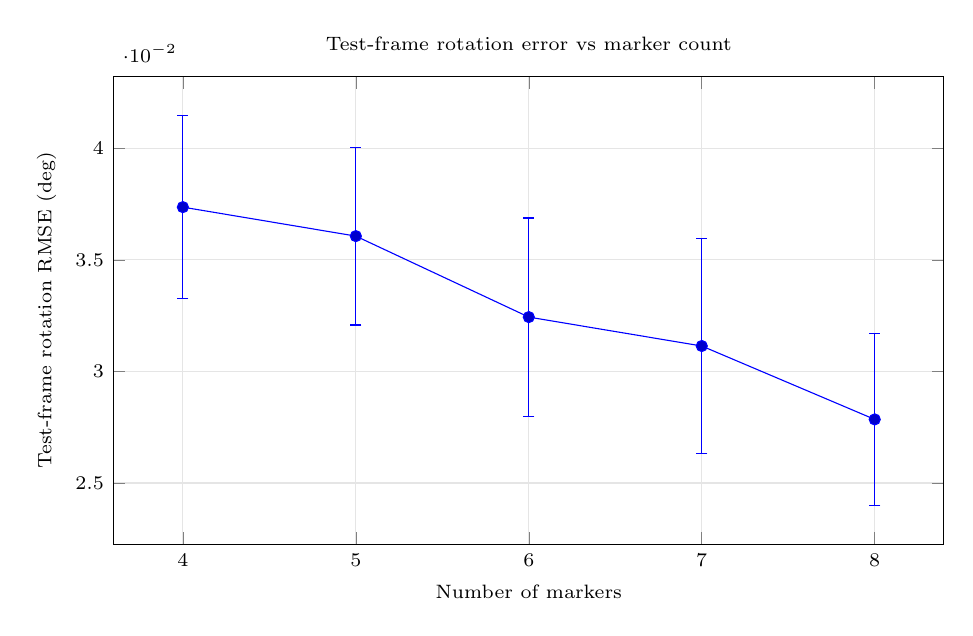
\begin{tikzpicture}
\begin{axis}[
  width=\linewidth,height=0.62\linewidth,
  title={Test-frame rotation error vs marker count},
  xlabel={Number of markers},ylabel={Test-frame rotation RMSE (deg)},
  xtick={4,5,6,7,8},grid=major,grid style={gray!20},
  title style={font=\scriptsize},label style={font=\scriptsize},
  tick label style={font=\scriptsize}]
\addplot+[blue,mark=*,error bars/.cd,y dir=both,y explicit]
table[x=x,y=y,y error=err] {
x y err
4 0.037363096 0.004098812
5 0.036063717 0.003985379
6 0.032434597 0.004442092
7 0.031137727 0.004800002
8 0.027848056 0.003844939
};
\end{axis}
\end{tikzpicture}
\end{minipage}\hfill
\begin{minipage}{0.49\textwidth}
\centering
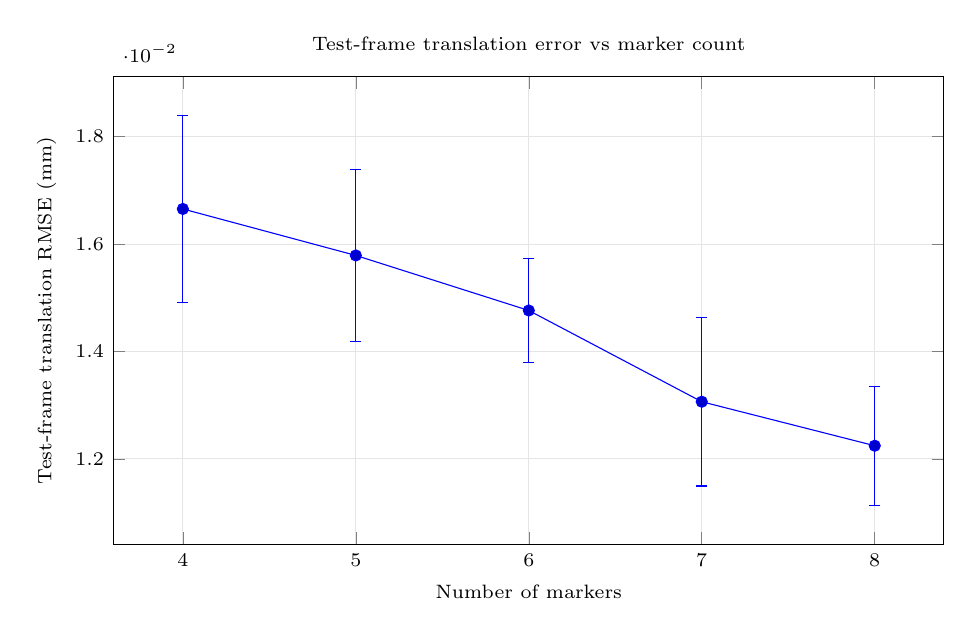
\begin{tikzpicture}
\begin{axis}[
  width=\linewidth,height=0.62\linewidth,
  title={Test-frame translation error vs marker count},
  xlabel={Number of markers},ylabel={Test-frame translation RMSE (mm)},
  xtick={4,5,6,7,8},grid=major,grid style={gray!20},
  title style={font=\scriptsize},label style={font=\scriptsize},
  tick label style={font=\scriptsize}]
\addplot+[blue,mark=*,error bars/.cd,y dir=both,y explicit]
table[x=x,y=y,y error=err] {
x y err
4 0.016654042 0.001736866
5 0.015788502 0.001599236
6 0.014763514 0.000967221
7 0.013064507 0.001569529
8 0.012245250 0.001106764
};
\end{axis}
\end{tikzpicture}
\end{minipage}
\caption{Frame error versus marker count and layout (A.4).}
\label{fig:validation-marker-count-layout}
\end{figure}

\subsubsection*{A.5 Marker-radius sensitivity}
For the fixed five-marker topology,
Figure~\ref{fig:validation-marker-radius} shows rotation RMSE decreasing from
$0.03606^\circ$ at $30\,\mathrm{mm}$ to $0.00435^\circ$ at
$250\,\mathrm{mm}$, approximately following $1/R_m$.  Translation RMSE
remains approximately $0.01579\,\mathrm{mm}$ in these trials.  This supports
the rotational benefit of spreading the markers without implying that radius
alone removes every source of tip-position error.

The triangular-bipyramid topology, ten training observations, and three
refinement passes remain fixed.  Points and error bars show the mean and one
sample standard deviation across eight seeds.  Only test-frame rotation RMSE
is plotted; translation and marker-coordinate errors are not shown.

\begin{figure}[H]
\centering
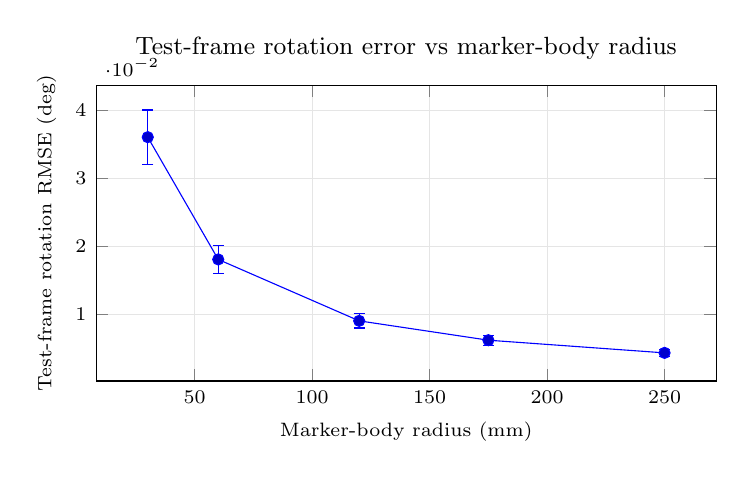
\begin{tikzpicture}
\begin{axis}[
  width=0.78\textwidth,height=0.44\textwidth,
  title={Test-frame rotation error vs marker-body radius},
  xlabel={Marker-body radius (mm)},
  ylabel={Test-frame rotation RMSE (deg)},
  grid=major,grid style={gray!20},
  title style={font=\small},label style={font=\scriptsize},
  tick label style={font=\scriptsize}]
\addplot+[blue,mark=*,error bars/.cd,y dir=both,y explicit]
table[x=x,y=y,y error=err] {
x y err
30  0.036063717 0.003985379
60  0.018086473 0.002066554
120 0.009056533 0.001052116
175 0.006213025 0.000725545
250 0.004350407 0.000509763
};
\end{axis}
\end{tikzpicture}
\caption{Rotation error versus marker-body radius (A.5).}
\label{fig:validation-marker-radius}
\end{figure}

\subsection{Unit Test B: tip calibration}
Unit Test B evaluates the \path{compute_pivot_calibration} function, which
estimates the pointer-tip coordinates and their covariance from paired frames
and sensor readings.  Tests B.1--B.7 assess exact recovery, invalid-input
handling, observation-count sensitivity, sensor filtering, the minimum valid
sample count, frame-error propagation, and covariance calculation.
Calibration error is measured as
\begin{equation}
e_{\mathrm{tip}}
=\norm{\widehat{\vct p}_{\mathrm{tip}}-\vct p_{\mathrm{tip}}^*}.
\end{equation}

\subsubsection*{B.1 Exact synthetic tip recovery}
Exact paired frames and exact sensor readings recover the known tip
$[1.5,-0.75,-149]^T\,\mathrm{mm}$ to below $10^{-14}\,\mathrm{mm}$ per
axis.  This deterministic case checks transform direction and least-squares
recovery without measurement noise.

\subsubsection*{B.2 Invalid calibration inputs}
All six malformed-input tests raise \path{ValueError}: mismatched list lengths,
non-\path{Frame} inputs, nonorthogonal rotations, singular rotations,
nonfinite frames, and invalid sensor types.  These checks distinguish
interface errors from physically unusable sensor readings.

\subsubsection*{B.3 Calibration observation-count sensitivity}
Figure~\ref{fig:validation-calibration-count} shows mean tip error falling from
$1.32716$ to $0.24062\,\mathrm{mm}$ as the valid observation count rises from
2 to 60.  The trend is approximately consistent with the normalized
$1/\sqrt N$ reference under these independent frame perturbations.  Error
bars show the sample standard deviation across 40 seeds; they are not
confidence intervals and do not establish a universal error bound.

Exact sensor readings are combined with independently perturbed pointer and
calibration frames at a fixed perturbation strength.  Points show the mean
across 40 seeds.  The dashed $1/\sqrt N$ reference is normalized to the first
measured mean and serves only as a descriptive comparison.

\begin{figure}[H]
\centering
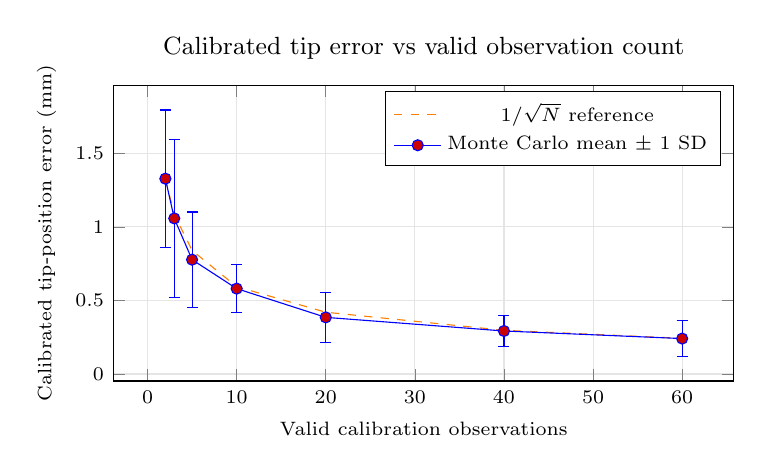
\begin{tikzpicture}
\begin{axis}[
  width=0.78\textwidth,height=0.44\textwidth,
  title={Calibrated tip error vs valid observation count},
  xlabel={Valid calibration observations},
  ylabel={Calibrated tip-position error (mm)},
  grid=major,grid style={gray!20},
  title style={font=\small},label style={font=\scriptsize},
  tick label style={font=\scriptsize},
  legend style={font=\scriptsize,at={(0.98,0.98)},anchor=north east}]
\addplot+[orange,dashed,mark=none] coordinates {
(2,1.3271574) (3,1.0836195) (5,0.8393681) (10,0.5935228)
(20,0.4196840) (40,0.2967614) (60,0.2423047)};
\addlegendentry{$1/\sqrt{N}$ reference}
\addplot+[blue,mark=*,error bars/.cd,y dir=both,y explicit]
table[x=x,y=y,y error=err] {
x y err
2  1.3271574 0.4662160
3  1.0572478 0.5389133
5  0.7766543 0.3242295
10 0.5800715 0.1611879
20 0.3847907 0.1707120
40 0.2921166 0.1071552
60 0.2406156 0.1207642
};
\addlegendentry{Monte Carlo mean $\pm$ 1 SD}
\end{axis}
\end{tikzpicture}
\caption{Tip error versus calibration observation count (B.3).}
\label{fig:validation-calibration-count}
\end{figure}

\subsubsection*{B.4 Invalid sensor filtering}
Three tests verify that the assignment sentinel
$[-10000,-10000,-10000]^T$ is discarded with its paired frames, a reading at
exactly $5\,\mathrm{mm}$ remains valid, and missing or nonfinite readings
(\path{None}, NaN, or infinity) are ignored.  Valid observations still recover
the known tip after unusable records are appended.

\subsubsection*{B.5 Minimum valid observation count}
Zero or one valid reading is rejected, while two valid readings return the
calibrated tip and a $3\times3$ covariance.  One proper rotation is
mathematically sufficient to determine the three tip coordinates; the
two-observation minimum is imposed to estimate empirical covariance.  Invalid
sensor records do not count toward this minimum.

\subsubsection*{B.6 Frame-error propagation into tip calibration}
The observation count is fixed at 15, and the sensor readings remain exact.
Figure~\ref{fig:validation-frame-error-propagation} reports means and sample
standard deviations across 20 seeds while perturbing the pointer and
calibration frames independently.  These trials begin with frame estimates;
marker refinement and SVD registration are not rerun in this study.

\noindent\textbf{B.6.1 Frame-rotation-error propagation.}
Increasing the per-axis rotation standard deviation of the left-multiplied
perturbation from $0.10^\circ$ to $1.00^\circ$ increases the mean tip error
from $0.38781$ to $3.91504\,\mathrm{mm}$ (left panel).  The explicit
translation component of the perturbation is zero.

\noindent\textbf{B.6.2 Frame-translation-error propagation.}
With identity perturbation rotation, increasing per-axis translation standard
deviation from $0.10$ to $1.00\,\mathrm{mm}$ increases mean tip error from
$0.05292$ to $0.52916\,\mathrm{mm}$ (right panel).  The two sweeps use
different perturbation units and ranges; they do not provide a dimensionless
ranking of rotation and translation sensitivity.

The implementation uses $\widehat F=\Delta F F$, so
$\widehat R=R_{\Delta}R$ and
$\widehat{\vct t}=R_{\Delta}\vct t+\vct t_{\Delta}$.  Consequently, the
rotation sweep also changes frame-origin coordinates even when
$\vct t_{\Delta}=0$.  Its result includes this coordinate-dependent effect
and should not be described as a rotation-only change at fixed translation or
attributed solely to the pointer-tip lever arm.

\begin{figure}[H]
\centering
\begin{minipage}{0.49\textwidth}
\centering
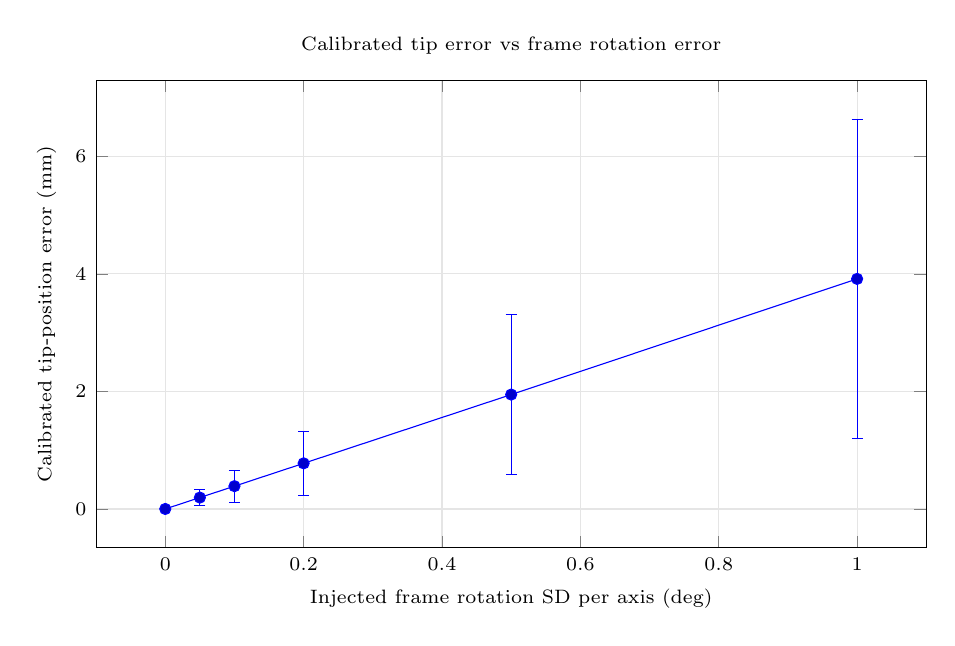
\begin{tikzpicture}
\begin{axis}[
  width=\linewidth,height=0.62\linewidth,
  title={Calibrated tip error vs frame rotation error},
  xlabel={Injected frame rotation SD per axis (deg)},
  ylabel={Calibrated tip-position error (mm)},
  grid=major,grid style={gray!20},
  title style={font=\scriptsize},label style={font=\scriptsize},
  tick label style={font=\scriptsize}]
\addplot+[blue,mark=*,error bars/.cd,y dir=both,y explicit]
table[x=x,y=y,y error=err] {
x y err
0    0          0
0.05 0.19381802 0.13598363
0.10 0.38780971 0.27194885
0.20 0.77633449 0.54381361
0.50 1.94660196 1.35869889
1.00 3.91503790 2.71330473
};
\end{axis}
\end{tikzpicture}
\end{minipage}\hfill
\begin{minipage}{0.49\textwidth}
\centering
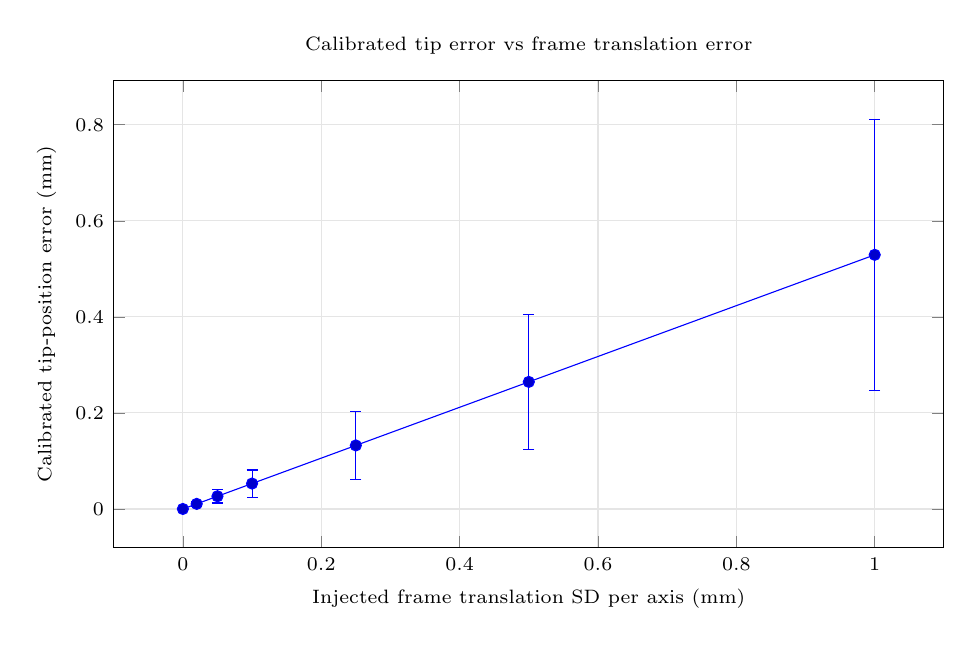
\begin{tikzpicture}
\begin{axis}[
  width=\linewidth,height=0.62\linewidth,
  title={Calibrated tip error vs frame translation error},
  xlabel={Injected frame translation SD per axis (mm)},
  ylabel={Calibrated tip-position error (mm)},
  grid=major,grid style={gray!20},
  title style={font=\scriptsize},label style={font=\scriptsize},
  tick label style={font=\scriptsize}]
\addplot+[blue,mark=*,error bars/.cd,y dir=both,y explicit]
table[x=x,y=y,y error=err] {
x y err
0    0          0
0.02 0.01058315 0.00563789
0.05 0.02645787 0.01409472
0.10 0.05291573 0.02818944
0.25 0.13228933 0.07047359
0.50 0.26457866 0.14094719
1.00 0.52915731 0.28189437
};
\end{axis}
\end{tikzpicture}
\end{minipage}
\caption{Frame-error propagation into tip calibration (B.6).}
\label{fig:validation-frame-error-propagation}
\end{figure}

\subsubsection*{B.7 Covariance calculation}
Two analytic tests check the covariance calculation.  Identical
single-observation tip estimates give a zero covariance matrix.  Estimates
with $x$ offsets of $-1$, 0, and $+1\,\mathrm{mm}$ have sample variance
$1\,\mathrm{mm}^2$; the covariance of their three-sample mean is therefore
\begin{equation}
C_{\mathrm{tip}}=\diag(1/3,0,0)\ \mathrm{mm}^2.
\end{equation}
The computed matrix agrees with this analytic result.

\subsection{Limitations}
All deterministic tests pass, but the sensitivity results apply only to the
stated seed sets and the result for the 102 poses within $45^\circ$ is one simulation
realization.  Empirical tip covariance also excludes marker-model bias shared
across observations.  The reported pass rates are therefore empirical results,
not guarantees for every admissible pose.

\section{Result}
\subsection{Marker-refinement result}
Refinement updates the nominal local marker coordinates before calibration and
testing.  Table~\ref{tab:result-refinement} reports the magnitude
$\norm{\widehat{\vct a}_{m,k}^{(N_r)}-\vct a_{m,k}}$ for each marker.  These
values are model updates, not errors relative to hidden ground truth.

\begin{table}[H]
\centering
\small
\caption{Marker-coordinate updates after refinement [mm].}
\label{tab:result-refinement}
\begin{tabular}{lrrrrrr}
\toprule
Body & M1 & M2 & M3 & M4 & M5 & Mean \\
\midrule
Pointer & 0.939 & 1.803 & 0.714 & 0.924 & 1.456 & 1.167 \\
Calibration & 0.652 & 0.435 & 0.536 & 0.812 & 0.588 & 0.605 \\
Nearby & 0.863 & 1.489 & 1.147 & 1.167 & 0.944 & 1.122 \\
\bottomrule
\end{tabular}
\end{table}

\subsection{Calibrated-tip result}
From 60 valid observations, calibration produces the tip coordinate in the
pointer frame:
\begin{equation}
\widehat{\vct p}_{\mathrm{tip}}
=[1.362,-4.432,-149.684]^T\ \mathrm{mm}.
\end{equation}
Its estimated covariance and per-axis standard deviation are
\begin{equation}
\widehat C_{\mathrm{tip}}
=\begin{bmatrix}
0.001&0&0.001\\
0&0.002&0\\
0.001&0&0.002
\end{bmatrix}\ \mathrm{mm}^2,
\qquad
\vct{\sigma}_{\mathrm{tip}}
=[0.037,0.047,0.047]^T\ \mathrm{mm}.
\end{equation}
This pointer-frame vector is the calibrated input used by Step~8; it is not a
single position representing all test poses.

\subsection{Step~8 test result}
For test pose $i$, the program predicts
$\widehat{\vct p}_{t,\mathrm{near},i}$ in the nearby frame.  All reported poses use Euler-angle components from
$\Theta=\{0,\pm\pi/6,\pm\pi/3,\pm\pi/2\}$ and have an actual
pointer-axis tilt of at most $45^\circ$.  There are $N_{45}=102$ such poses,
\begin{equation}
\Delta\vct p_i
=\widehat{\vct p}_{t,\mathrm{near},i}
-\vct p_{t,\mathrm{near},i}^*,
\end{equation}
and the empirical mean and sample covariance are
\begin{equation}
\overline{\Delta\vct p}_{45}
=[0.044,-0.546,0.998]^T\ \mathrm{mm},
\qquad
\widehat C_{\Delta p,45}
=\begin{bmatrix}
0.203&-0.036&-0.049\\
-0.036&0.170&-0.109\\
-0.049&-0.109&0.100
\end{bmatrix}\ \mathrm{mm}^2.
\end{equation}

\begin{table}[H]
\centering
\small
\caption{Nearby-frame tip errors within $45^\circ$ of vertical.}
\label{tab:result-summary}
\begin{tabular}{rrrrr}
\toprule
$N_{45}$ & Mean [mm] & RMSE [mm] & Maximum [mm] & Within $2\,\mathrm{mm}$ \\
\midrule
102 & 1.260 & 1.329 & 2.155 & 96.1\% \\
\bottomrule
\end{tabular}
\end{table}
The assignment-required region achieves a $96.1\%$ empirical pass rate.  In
the nearby-size comparison, the $500\,\mathrm{mm}$ candidate gives an RMSE
of $1.022\,\mathrm{mm}$, a maximum error of $1.890\,\mathrm{mm}$, and a
$100\%$ pass rate over these poses.

\section{AI Assistance and Use of Tools}
AI assistance was used to check code and support mathematical derivations;
OpenAI Codex also assisted with notebook comparison and report preparation.
The prompts requested code checks and help with formula derivations, a
block-by-block comparison with the unfinished notebook, and advice on placing
the unit-test plots in the report.  Follow-up prompts requested insertion of
the plots with captions, A.1--A.5 and B.1--B.7 headings, consistent table
fonts, a shorter repository reference, correction of Figure~4, and a full
formatting review.  AI-assisted explanatory text and LaTeX edits were
incorporated into the report; the numerical plot data came from saved notebook
outputs, and LaTeX/Tectonic was used to compile and inspect the PDF.

\clearpage
\begin{thebibliography}{99}
\bibitem{assignment} R. H. Taylor, \emph{Assignment 1 -- CIS I (601.455/655), Fall 2026}, September 24, 2026, pp. 2--7, \texttt{2026\_assignment\_1\_.pdf}.
\bibitem{calibration} R. H. Taylor, \emph{Calibration}, CIS I lecture notes, Fall 2026, slides 7--15.
\bibitem{leastsquares} R. H. Taylor, \emph{Linear Least Squares Review}, CIS I lecture notes, Fall 2026, slides 1--10.
\bibitem{repo} LCSR-CIIS, \emph{CIS I Course repository}.
\url{https://github.com/LCSR-CIIS/CIS_I_Course}.
\bibitem{ndiSphere} Northern Digital Inc., \emph{NDI Passive Spheres},
11.8-mm passive marker sphere specification, accessed October 10, 2026.
\url{https://www.ndigital.com/polaris/ndi-passive-sphere/}.
\bibitem{pointerReview} K. R\'acz, B. Sereg\'ely, and R. M. Kiss,
``Performance of optically tracked instrumented pointers: a systematic
literature review,'' \emph{Biomedical Engineering Online}, vol.~24, art.~142,
2025.
\url{https://pmc.ncbi.nlm.nih.gov/articles/PMC12676873/}.
\bibitem{openDRF} A. Manbachi, J. H. Siewerdsen, et al., ``Design and
validation of an open-source library of dynamic reference frames for research
and education in optical tracking,'' \emph{Journal of Medical Imaging},
vol.~5, no.~2, 2018.
\url{https://pmc.ncbi.nlm.nih.gov/articles/PMC5806031/}.
\end{thebibliography}
\end{document}
